\documentclass[3p,super,numbers,sort&compress,10pt]{elsarticle}
\let\labelindent\relax
\usepackage{enumitem}
\usepackage{etex}
\usepackage{amssymb,amsfonts,amsmath,amsthm}
\usepackage{graphicx}
\usepackage[usenames,x11names, dvipsnames, svgnames]{xcolor}
\usepackage{amsmath,amssymb}
\usepackage{dsfont}
\usepackage{amsfonts}
\usepackage{mathrsfs}
\usepackage{texshade}
\usepackage{multirow}
\usepackage{hyperref}
\hypersetup{
  colorlinks=true,
  linkcolor=black,
  citecolor=black,
  filecolor=black,
  urlcolor=DodgerBlue4,
  breaklinks=false,
  % linkbordercolor=red,% hyperlink borders will be red
  % pdfborderstyle={/S/U/W 1}% border style will be underline of width 1pt
}
\usepackage{array}
\usepackage{xr}
\usepackage{verbatim}
% \usepackage{multirow}    
% \usepackage[T1,euler-digits]{eulervm}
% \usepackage{times}
% \usepackage{pxfonts}
\usepackage{tikz}
\usepackage{pgfplots}
\usetikzlibrary{shapes,calc,shadows,fadings,arrows,decorations.pathreplacing,automata,positioning}
\usetikzlibrary{external}
\usetikzlibrary{decorations.text}
\usepgfplotslibrary{colorbrewer} 

\tikzexternalize[prefix=./Figures/External/]% activate externalization!
\tikzexternaldisable
% \addtolength{\voffset}{.1in}  
\usepackage{geometry}
\geometry{a4paper, left=.65in,right=.65in,top=.8in,bottom=0.7in}

\addtolength{\textwidth}{-.1in}    
\addtolength{\hoffset}{.05in}    
\addtolength{\textheight}{0in}    
\addtolength{\footskip}{0in}    
\usepackage{rotating}
\definecolor{nodecol}{RGB}{240,240,220}
\definecolor{nodeedge}{RGB}{240,240,225}
\definecolor{edgecol}{RGB}{130,130,130}
\tikzset{%
  fshadow/.style={      preaction={
      fill=black,opacity=.3,
      path fading=circle with fuzzy edge 20 percent,
      transform canvas={xshift=1mm,yshift=-1mm}
    }} 
}
\usetikzlibrary{pgfplots.dateplot}
\usetikzlibrary{patterns}
\usetikzlibrary{decorations.markings}
\usepackage{fancyhdr}
\usepackage{mathtools}
\usepackage{datetime}
\usepackage{comment}
%% ## Equation Space Control---------------------------
\def\EQSP{3pt}
\newcommand{\mltlne}[2][\EQSP]{\begingroup\setlength\abovedisplayskip{#1}\setlength\belowdisplayskip{#1}\begin{equation}\begin{multlined} #2 \end{multlined}\end{equation}\endgroup\noindent}
\newcommand{\cgather}[2][\EQSP]{\begingroup\setlength\abovedisplayskip{#1}\setlength\belowdisplayskip{#1}\begin{gather} #2 \end{gather}\endgroup\noindent}
\newcommand{\cgathers}[2][\EQSP]{\begingroup\setlength\abovedisplayskip{#1}\setlength\belowdisplayskip{#1}\begin{gather*} #2 \end{gather*}\endgroup\noindent}
\newcommand{\calign}[2][\EQSP]{\begingroup\setlength\abovedisplayskip{#1}\setlength\belowdisplayskip{#1}\begin{align} #2 \end{align}\endgroup\noindent}
\newcommand{\caligns}[2][\EQSP]{\begingroup\setlength\abovedisplayskip{#1}\setlength\belowdisplayskip{#1}\begin{align*} #2 \end{align*}\endgroup\noindent}
\newcommand{\mnp}[2]{\begin{minipage}{#1}#2\end{minipage}} 
%% COLOR DEFS------------------------------------------
\newtheorem{thm}{Theorem}
\newtheorem{cor}{Corollary}
\newtheorem{lem}{Lemma}
\newtheorem{prop}{Proposition}
\newtheorem{defn}{Definition}
\newtheorem{exmpl}{Example}
\newtheorem{rem}{Remark}
\newtheorem{notn}{Notation}
%% ------------PROOF INCLUSION -----------------
\def\NOPROOF{Proof omitted.}
\newif\ifproof
\prooffalse % or \draftfalse
\newcommand{\Proof}[1]{
  \ifproof
  \begin{IEEEproof}
    #1\end{IEEEproof}
  \else
  \NOPROOF
  \fi
}
%% ------------ -----------------
\newcommand{\DETAILS}[1]{#1}
%% ------------ -----------------
% color commands------------------------
\newcommand{\etal}{\textit{et} \mspace{3mu} \textit{al.}}
% \renewcommand{\algorithmiccomment}[1]{$/** $ #1 $ **/$}
\newcommand{\vect}[1]{\textbf{\textit{#1}}}
\newcommand{\figfont}{\fontsize{8}{8}\selectfont\strut}
\newcommand{\hlt}{ \bf \sffamily \itshape\color[rgb]{.1,.2,.45}}
\newcommand{\pitilde}{\widetilde{\pi}}
\newcommand{\Pitilde}{\widetilde{\Pi}}
\newcommand{\bvec}{\vartheta}
\newcommand{\algo}{\textrm{\bf\texttt{GenESeSS}}\xspace}
\newcommand{\xalgo}{\textrm{\bf\texttt{xGenESeSS}}\xspace}
\newcommand{\FNTST}{\bf }
\newcommand{\FNTED}{\color{darkgray} \scriptsize $\phantom{.}$}
\renewcommand{\baselinestretch}{.95}
\newcommand{\sync}{\otimes}
\newcommand{\psync}{\hspace{3pt}\overrightarrow{\hspace{-3pt}\sync}}
% \newcommand{\psync}{\raisebox{-4pt}{\begin{tikzpicture}\node[anchor=south] (A) {$\sync$};
%   \draw [->,>=stealth] ([yshift=-2pt, xshift=2pt]A.north west) -- ([yshift=-2pt]A.north east); %\end{tikzpicture}}}
\newcommand{\base}[1]{\llbracket #1 \rrbracket}
\newcommand{\nst}{\textrm{\sffamily\textsc{Numstates}}}
\newcommand{\HA}{\boldsymbol{\mathds{H}}}
\newcommand{\eqp}{ \vartheta }
\newcommand{\entropy}[1]{\boldsymbol{h}\left ( #1 \right )}
\newcommand{\norm}[1]{\left\lVert #1 \right\rVert}%
\newcommand{\abs}[1]{\left\lvert #1 \right\rvert}%
\newcommand{\absB}[1]{\big\lvert #1 \big\rvert}%
% #############################################################
% #############################################################
% PREAMBLE ####################################################
% #############################################################
% #############################################################
% \usepackage{pnastwoF}      
\DeclareMathOperator*{\argmax}{argmax}
\DeclareMathOperator*{\argmin}{arg\,min}
\DeclareMathOperator*{\expect}{\mathbf{E}}
\DeclareMathOperator*{\var}{\mathbf{Var}}

\newcommand{\ND}{ \mathcal{N}  }
\usepackage[linesnumbered,ruled,vlined,noend]{algorithm2e}
\newcommand{\captionN}[1]{\caption{\color{darkgray} \sffamily \fontsize{9}{11}\selectfont #1  }}
\newcommand{\btl}{\ \textbf{\small\sffamily bits/letter}}
\usepackage{txfonts}
% \usepackage{ccfonts}
%%% save defaults
\renewcommand{\rmdefault}{phv} % Arial
\renewcommand{\sfdefault}{phv} % Arial
\edef\keptrmdefault{\rmdefault}
\edef\keptsfdefault{\sfdefault}
\edef\keptttdefault{\ttdefault}

% \usepackage{kerkis}
\usepackage[OT1]{fontenc}
\usepackage{concmath}
% \usepackage[T1]{eulervm} 
% \usepackage[OT1]{fontenc}
%%% restore defaults
\edef\rmdefault{\keptrmdefault}
\edef\sfdefault{\keptsfdefault}
\edef\ttdefault{\keptttdefault}
\tikzexternalenable
% ##########################################################
\tikzfading[name=fade out,
inner color=transparent!0,
outer color=transparent!100]
% ###################################
\newcommand{\xtitaut}[2]{
  \noindent\mnp{\textwidth}{
    \mnp{\textwidth}{\raggedright\Huge \bf \sffamily #1}

    \vskip 1em

    {\bf \sffamily #2}
  }
  \vskip 2em
}
% ###################################
% ###################################
\tikzset{wiggle/.style={decorate, decoration={random steps, amplitude=10pt}}}
\usetikzlibrary{decorations.pathmorphing}
\pgfdeclaredecoration{Snake}{initial}
{
  \state{initial}[switch if less than=+.625\pgfdecorationsegmentlength to final,
  width=+.3125\pgfdecorationsegmentlength,
  next state=down]{
    \pgfpathmoveto{\pgfqpoint{0pt}{\pgfdecorationsegmentamplitude}}
  }
  \state{down}[switch if less than=+.8125\pgfdecorationsegmentlength to end down,
  width=+.5\pgfdecorationsegmentlength,
  next state=up]{
    \pgfpathcosine{\pgfqpoint{.25\pgfdecorationsegmentlength}{-1\pgfdecorationsegmentamplitude}}
    \pgfpathsine{\pgfqpoint{.25\pgfdecorationsegmentlength}{-1\pgfdecorationsegmentamplitude}}
  }
  \state{up}[switch if less than=+.8125\pgfdecorationsegmentlength to end up,
  width=+.5\pgfdecorationsegmentlength,
  next state=down]{
    \pgfpathcosine{\pgfqpoint{.25\pgfdecorationsegmentlength}{\pgfdecorationsegmentamplitude}}
    \pgfpathsine{\pgfqpoint{.25\pgfdecorationsegmentlength}{\pgfdecorationsegmentamplitude}}
  }
  \state{end down}[width=+.3125\pgfdecorationsegmentlength,
  next state=final]{
    \pgfpathcosine{\pgfqpoint{.15625\pgfdecorationsegmentlength}{-.5\pgfdecorationsegmentamplitude}}
    \pgfpathsine{\pgfqpoint{.15625\pgfdecorationsegmentlength}{-.5\pgfdecorationsegmentamplitude}}
  }
  \state{end up}[width=+.3125\pgfdecorationsegmentlength,
  next state=final]{
    \pgfpathcosine{\pgfqpoint{.15625\pgfdecorationsegmentlength}{.5\pgfdecorationsegmentamplitude}}
    \pgfpathsine{\pgfqpoint{.15625\pgfdecorationsegmentlength}{.5\pgfdecorationsegmentamplitude}}
  }
  \state{final}{\pgfpathlineto{\pgfpointdecoratedpathlast}}
}
% ###################################
% ###################################
\newcolumntype{L}[1]{>{\rule{0pt}{2ex}\raggedright\let\newline\\\arraybackslash\hspace{0pt}}m{#1}}
\newcolumntype{C}[1]{>{\rule{0pt}{2ex}\centering\let\newline\\\arraybackslash\hspace{0pt}}m{#1}}
\newcolumntype{R}[1]{>{\rule{0pt}{2ex}\raggedleft\let\newline\\\arraybackslash\hspace{0pt}}m{#1}}




\newcommand{\drhh}[8]{
  \begin{axis}[semithick,
    font=\bf \sffamily \fontsize{7}{7}\selectfont,
    name=H2,
    at=(#4), anchor=#5,
    xshift=.3in,
    yshift=-.3in,
    width=\WDT, 
    height=\HGT, 
    title={{\LARGE G } ROC area distribution (Out-of-sample)}, 
    title style={align=right, },legend cell align=left,
    legend style={ xshift=3.5in, yshift=-.6in, draw=white, fill= gray, fill opacity=0.2, 
      text opacity=1,},
    axis line style={black!80, opacity=0,   thick,,ultra thin, rounded corners=0pt},
    axis on top=false, 
    xlabel={ROC area},
    ylabel={probability},
    ylabel style={yshift=-.25in},
    xlabel style={yshift=.1in},
    grid style={dashed, gray!50},
    % grid,
    axis background/.style={top color=gray!1,bottom color=gray!2},
    enlargelimits=false, 
    scale only axis=true,
    ymin=0,
    % xmin=.7,xmax=1.0,
    ylabel style={yshift=.05in},
    major tick length=0pt,yticklabel style={/pgf/number format/fixed,/pgf/number format/precision=2},xticklabel style={/pgf/number format/fixed,/pgf/number format/precision=2},
    #7,
    ]
    \addplot [
    fill=#8,
    thick,
    draw=white,
    opacity=1,
    hist={density,bins=10},
    ] table [y index=#3] {#1};
    % \addlegendentry{$\Delta$ ROC};
    \addplot [very thick, Red2,, opacity=.95] gnuplot [raw gnuplot] {plot '#1' u #2:(1./#6.) smooth kdensity};
    % 
    % \draw[thin,black ] (axis cs:.89291,\pgfkeysvalueof{/pgfplots/ymin}) -- (axis cs:.89291,\pgfkeysvalueof{/pgfplots/ymax}) node [midway,right, pos=0.2] {89.3\%};
    % \addlegendentry{kde};
  \end{axis}
}


\newcommand{\erhh}[6]{
  \begin{axis}[semithick,
    font=\bf \sffamily \fontsize{7}{7}\selectfont,
    name=H2,
    at=(#3), anchor=#4,
    xshift=.3in,
    yshift=-.3in,
    width=\WDT, 
    height=\HGT, 
    title style={align=center, },legend cell align=left,
    legend style={ xshift=3.5in, yshift=-.6in, draw=white, fill= gray, fill opacity=0.2, 
      text opacity=1,},
    axis line style={black!80, opacity=0,   thick,,ultra thin, rounded corners=0pt},
    axis on top=false, 
    xlabel={ROC area},
    ylabel={probability},
    ylabel style={yshift=-.25in},
    xlabel style={yshift=.1in},
    grid style={dashed, gray!50},
    % grid,
    axis background/.style={top color=gray!1,bottom color=gray!2},
    enlargelimits=false, 
    scale only axis=true,
    % ymin=0, 
    % xmin=.7,xmax=1.0,
    ylabel style={yshift=.05in},
    major tick length=0pt,yticklabel style={/pgf/number format/fixed,/pgf/number format/precision=2},xticklabel style={/pgf/number format/fixed,/pgf/number format/precision=2},
    #5,
    ]
    \addplot[semithick, #6]
    table[x expr=(\coordindex+1),y expr=(\thisrowno{#2})] {#1};
    % \addlegendentry{Cullman, Alabama};
  \end{axis}
}
% ################################################
% ################################################
% ################################################
% ################################################
\def\DISCLOSURE#1{\def\disclosure{#1}}
\DISCLOSURE{\raisebox{15pt}{$\phantom{XxxX}$This sheet contains proprietary information 
    not to be released to third parties except for the explicit purpose of evaluation.}
}
% ####################################
\newcommand{\set}[1]{\left\{ #1 \right\}}
\newcommand{\paren}[1]{\left( #1 \right)}
\newcommand{\bracket}[1]{\left[ #1 \right]}
% \newcommand{\norm}[1]{\left\Vert #1 \right\Vert}
\newcommand{\nrm}[1]{\left\llbracket{#1}\right\rrbracket}
\newcommand{\parenBar}[2]{\paren{#1\,{\left\Vert\,#2\right.}}}
\newcommand{\parenBarl}[2]{\paren{\left.#1\,\right\Vert\,#2}}
\newcommand{\ie}{$i.e.$\xspace}
\newcommand{\addcitation}{\textcolor{black!50!red}{\textbf{ADD CITATION}}}
\newcommand{\subtochange}[1]{{\color{black!50!green}{#1}}}
\newcommand{\tobecompleted}{{\color{black!50!red}TO BE COMPLETED.}}


\newcommand{\pIn}{\mathscr{P}_{\textrm{in}}}
\newcommand{\pOut}{\mathscr{P}_{\textrm{out}}}
\newcommand{\aIn}[1][\Sigma]{#1_{\textrm{in}}}
\newcommand{\aOut}[1][\Sigma]{#1_{\textrm{out}}}
\newcommand{\xin}[1]{#1_{\textrm{in}}}
\newcommand{\xout}[1]{#1_{\textrm{out}}}

\newcommand{\R}{\mathbb{R}} % Set of real numbers
\newcommand{\F}[1][]{\mathcal{F}_{#1}}
\newcommand{\SR}{\mathcal{S}} % Semiring of sets
\newcommand{\RR}{\mathcal{R}} % Ring of sets
\newcommand{\N}{\mathbb{N}} % Set of natural numbers (0 included)


\newcommand{\Pp}[1][n]{\mathscr{P}^+_{#1}}
\renewcommand{\entropy}[1]{\boldsymbol{h}\left ( #1 \right )}



\makeatletter
\pgfdeclarepatternformonly[\hatchdistance,\hatchthickness]{flexible hatch}
{\pgfqpoint{0pt}{0pt}}
{\pgfqpoint{\hatchdistance}{\hatchdistance}}
{\pgfpoint{\hatchdistance-1pt}{\hatchdistance-1pt}}%
{
  \pgfsetcolor{\tikz@pattern@color}
  \pgfsetlinewidth{\hatchthickness}
  \pgfpathmoveto{\pgfqpoint{0pt}{0pt}}
  \pgfpathlineto{\pgfqpoint{\hatchdistance}{\hatchdistance}}
  \pgfusepath{stroke}
}
\makeatother

\pgfdeclarepatternformonly{north east lines wide}%
{\pgfqpoint{-1pt}{-1pt}}%
{\pgfqpoint{10pt}{10pt}}%
{\pgfqpoint{9pt}{9pt}}%
{
  \pgfsetlinewidth{0.7pt}
  \pgfpathmoveto{\pgfqpoint{0pt}{0pt}}
  \pgfpathlineto{\pgfqpoint{9.1pt}{9.1pt}}
  \pgfusepath{stroke}
}

\pgfdeclarepatternformonly{north west lines wide}%
{\pgfqpoint{-1pt}{-1pt}}%
{\pgfqpoint{10pt}{10pt}}%
{\pgfqpoint{9pt}{9pt}}%
{
  \pgfsetlinewidth{0.7pt}
  \pgfpathmoveto{\pgfqpoint{0pt}{9pt}}
  \pgfpathlineto{\pgfqpoint{9.1pt}{-0.1pt}}
  \pgfusepath{stroke}
}
\makeatletter

\pgfdeclarepatternformonly[\hatchdistance,\hatchthickness]{flexible hatchB}
{\pgfqpoint{0pt}{\hatchdistance}}
{\pgfqpoint{\hatchdistance}{0pt}}
{\pgfpoint{1pt}{\hatchdistance-1pt}}%
{
  \pgfsetcolor{\tikz@pattern@color}
  \pgfsetlinewidth{\hatchthickness}
  \pgfpathmoveto{\pgfqpoint{0pt}{\hatchdistance}}
  \pgfpathlineto{\pgfqpoint{\hatchdistance}{0pt}}
  \pgfusepath{stroke}
}    \makeatother


\def\TPR{\textrm{TPR}\xspace}
\def\TNR{\textrm{TNR}\xspace}
\def\FPR{\textrm{FPR}\xspace}
\def\PPV{\textrm{PPV}\xspace}

\usetikzlibrary{arrows.meta}
\usetikzlibrary{decorations.pathreplacing,shapes.misc}
\usepgfplotslibrary{fillbetween}
%\usepackage{tikz-network}
\usetikzlibrary{shapes.geometric}
\usetikzlibrary{math}
\usepgfplotslibrary{colorbrewer} 

\usepackage{textcomp}
\usepackage{colortbl}
\usepackage{array}
\usepackage{courier} 
\usepackage{wrapfig}
\usepackage{pifont}
\usetikzlibrary{chains,backgrounds}
\usetikzlibrary{intersections}
\usetikzlibrary{pgfplots.groupplots}
\usepgfplotslibrary{fillbetween} 
\usetikzlibrary{arrows.meta}
\usepackage{pgfplotstable}
%\usepackage[super,compress,sort,comma]{natbib}
\usepackage{setspace}
\usetikzlibrary{math}
\usetikzlibrary{matrix}
\usepackage{xstring}
\usepackage{xspace}
\usepackage{flushend}
\makeatletter
\renewcommand\section{\@startsection {section}{1}{\z@}%
  {-2ex \@plus -1ex \@minus -.2ex}%
  {1ex \@plus.1ex}%
  {\Large\bfseries\scshape}}
\renewcommand\subsection{\@startsection {section}{1}{\z@}%
  {-2ex \@plus -.25ex \@minus -.2ex}%
  {0.1ex \@plus.0ex}%
  {\fontsize{11}{10}\selectfont\bfseries\sffamily\color{black}}}
\renewcommand\subsubsection{\@startsection {section}{1}{\z@}%
  {0ex \@plus -.5ex \@minus -.2ex}%
  {0.0ex \@plus.5ex}%
  {\fontsize{9}{9}\selectfont\bfseries\itshape\sffamily\color{darkgray}}}
\renewcommand\paragraph{\@startsection {section}{1}{\z@}%
  {-.2ex \@plus -.5ex \@minus -.2ex}%
  {0.0ex \@plus.5ex}%
  {\fontsize{9}{9}\selectfont\itshape\sffamily\color{darkgray}}}
   
 
\makeatother
\makeatletter
\pgfdeclareradialshading[tikz@ball]{ball}{\pgfqpoint{-10bp}{10bp}}{%
  color(0bp)=(tikz@ball!30!white);
  color(9bp)=(tikz@ball!75!white);
  color(18bp)=(tikz@ball!90!black);
  color(25bp)=(tikz@ball!70!black);
  color(50bp)=(black)}
\makeatother
\newcommand{\tball}[1][CadetBlue4]{${\color{#1}\Large\boldsymbol{\blacksquare}}$}
\renewcommand{\baselinestretch}{1}
\renewcommand{\captionN}[1]{\caption{\color{CadetBlue4!50!black} \sffamily \fontsize{9}{10}\selectfont #1  }}
\tikzexternaldisable 
\parskip=6pt
\parindent=0pt
\newcommand{\Mark}[1]{\textsuperscript{#1}}
\pagestyle{fancy}

\newcounter{Dcounter}
\setcounter{Dcounter}{1}
\newcommand{\DQS}[1]{\ifdraftQ
{\marginpar{\tikzexternaldisable \tikz{\node[rounded corners=5pt,draw=none,thick,fill=black!10,font=\sffamily\fontsize{7}{8}\selectfont] {\mnp{.45in} {\color{Red3}\raggedright  \#\theDcounter.~#1}}; }}}\stepcounter{Dcounter}\xspace
\fi}

\newcommand{\qn}[1][i]{\Phi_{#1}}
\newcommand{\D}[1][i]{\mathscr{D}\left ( {\Sigma_#1} \right ) }
\newcommand{\Dx}{\mathscr{D}}
\def\J{\mathds{J}}
\def\M{\omega}
\def\N{\mathds{N}}
\newcommand{\cp}[1][P]{\langle #1 \rangle}
\newcommand{\mem}[1]{\M_{#1}} 
\usepackage[size=normal]{subcaption}
\makeatletter
\def\ps@pprintTitle{%
   \let\@oddhead\@empty
   \let\@evenhead\@empty
   \let\@oddfoot\@empty
   \let\@evenfoot\@oddfoot
}
\makeatother
\renewcommand{\baselinestretch}{1.05}
\externaldocument[SI-]{SI}
\newif\iftikzX
\tikzXtrue
\tikzXfalse
\newif\ifFIGS
\FIGSfalse  
\FIGStrue

\cfoot{\scriptsize\thepage}
\lfoot{}
\rfoot{}

  \def\MXCOL{black}
\def\FXCOL{Orchid3}
\def\MNCOL{SeaGreen4}
\def\FNCOL{SeaGreen4}
\def\NCOL{SeaGreen4}
\def\XCOL{Tomato}
\def\WCOL{Tomato}
\def\YCOL{DodgerBlue4} 
\def\XCOLA{\MXCOL}
\def\XCOLB{\FXCOL}
% ###########################################################
\def\treatment{positive\xspace}
\def\control{control\xspace}



\def\authora{Dmytro Onishchenko}
\def\authorb{Yi Huang}
\def\authorc{James van Horne}
\def\authord{Peter J. Smith}
\def\authore{Michael M. Msall}
\def\authorf{Ishanu Chattopadhyay}

\def\addressa{Department of Medicine, University of Chicago, Chicago, IL USA}
\def\addressb{Committee on Genetics, Genomics \& Systems Biology, University of Chicago, Chicago, IL USA}
\def\addressc{Committee on Quantitative Methods in Social, Behavioral, and Health Sciences, University of Chicago, Chicago, IL USA}
\def\addressd{Department of Pediatrics, Section of Developmental and Behavioral Pediatrics, University of Chicago, Chicago, IL USA}
\def\addresse{Department of Pediatrics, Section Chief of Developmental and Behavioral Pediatrics, University of Chicago, Chicago, IL USA}
\def\addressf{Joseph  P. Kennedy Research Center on Intellectual and Neurodevelopmental Disabilities, University of Chicago, Chicago, IL USA}
\def\addressg{Executive Committee Chair, American Academy of Pediatrics’ Section on Developmental and Behavioral Pediatrics}


\def\TITLE{Reduced False Positives in  Autism Screening Via  Digital  Bio-markers Inferred from Deep Co-morbidity Patterns}
\title{\TITLE}
\author{\sffamily  \fontsize{10}{12}\selectfont  \authora$^{1}$, \authorb$^{1}$, \authorc$^{1}$,  \authord$^{4,7}$, \authore$^{5,6}$ and \authorf$^{1,2,3\bigstar}$\\                                                                
\vspace{10pt}                                                                   
                                                                                
\sffamily  \fontsize{10}{12}\selectfont                                         
$^{1}$\addressa\\   
$^{2}$\addressb\\ 
$^{3}$\addressc\\                                                                    
$^{4}$\addressd\\                            
$^{5}$\addresse\\
$^{6}$\addressf\\
$^{7}$\addressg

\vskip 1em                                                                      
$^\bigstar$To whom correspondence should be addressed: e-mail: \texttt{ishanu@uchicago.edu}.}

 \def\acor{ACoR\xspace}
 
\tikzexternaldisable
\begin{document}
\begin{frontmatter}
  \title{\TITLE} 
  \author[ad1,ad2,ad3]{Ishanu Chattopadhyay, PhD\corref{cor1}}
  \author[ad1]{Dmytro Onishchenko, MS}
  \author[ad1]{Yi Huang, PhD}
  \author[ad1]{James van Horne, MS}
  \author[ad4,ad7]{Peter J. Smith, MD}
  \author[ad5,ad6]{Michael M. Msall, MD}

  \address[ad1]{Department of Medicine, University of Chicago, Chicago, IL, USA}
  \address[ad2]{Committee on Genetics, Genomics \& Systems Biology, University of Chicago, Chicago, IL, USA}
  \address[ad3]{Committee on Quantitative Methods in Social, Behavioral, and Health Sciences, University of Chicago, Chicago, IL, USA}
  \address[ad4]{Department of Pediatrics, Section of Developmental and Behavioral Pediatrics, University of Chicago, Chicago, IL, USA}
  \address[ad5]{Department of Pediatrics, Section Chief of Developmental and Behavioral Pediatrics, University of Chicago, Chicago, IL, USA}
  \address[ad6]{Joseph  P. Kennedy Research Center on Intellectual and Neurodevelopmental Disabilities, University of Chicago, Chicago, IL, USA}
  \address[ad7]{Executive Committee Chair, American Academy of Pediatrics’ Section on Developmental and Behavioral Pediatrics}

  \cortext[cor1]{To whom correspondence should be addressed: e-mail:  \texttt{ishanu@uchicago.edu}.}
  % ABSTRACT
\begin{abstract}
   Autism spectrum disorder (ASD) is a developmental disability associated with  significant social  and behavioral challenges. There is   a need for tools that help identify children with ASD as early as possible~\cite{cdc0,nimh}. Our current incomplete understanding of ASD pathogenesis, and the lack of reliable biomarkers hampers early detection,  intervention, and developmental trajectories. In this study we develop and validate  machine inferred digital biomarkers for autism using individual diagnostic codes already recorded during medical encounters. Our risk estimator  identifies  children at high risk  with a corresponding area under the receiver operating characteristic curve (AUC)  exceeding 80\% from shortly after two years of age for either sex, and across two independent databases of patient records. Thus, we systematically leverage ASD co-morbidities -  with no requirement of additional blood work, tests  or  procedures - to compute the Autism Co-morbid Risk Score (\acor) which predicts  elevated  risk  during the earliest childhood years, when interventions are the  most effective.  By itself, \acor has superior performance to common questionnaires-based screenings such as the M-CHAT/F~\cite{pmid31562252}, and has the potential to  reduce socio-economic, ethnic and demographic biases. In addition to standalone performance,  independence from questionnaire based screening allows us to further boost performance by conditioning on the individual M-CHAT/F scores --   we can either halve the false positive rate of current screening protocols or boost sensitivity to over 60\%, while maintaining  specificity  above 95\%.  Adopted  in practice, \acor could significantly reduce the median diagnostic age for ASD, and  reduce  long post-screen wait-times~\cite{pmid27565363}  experienced by families for confirmatory diagnoses and access to  evidence based interventions.
\end{abstract} 
\end{frontmatter}
%%%%%%%%%%%%%%%%%%%% 

\section*{Introduction}
% 
Autism spectrum disorder is a developmental disability associated with significant social  and behavioral challenges.
Even though ASD may be diagnosed as early as the  age of two~\cite{cdc},  children frequently remain undiagnosed  until after the fourth birthday~\cite{pmid24529515}. With genetic and metabolomic tests~\cite{howsmon2017classification,li2018high,hicks2018validation,smith2020metabolomics} still at their infancy,  a careful review of behavioral history and a direct
observation of symptoms is currently
necessary~\cite{volkmar2014practice,hyman2020identification} for a clinical diagnosis.  Starting with a positive initial screen, a confirmed diagnosis of ASD is a   multi-step process that often takes 3 months to 1 year,  delaying entry into time-critical intervention programs. While   lengthy evaluations~\cite{kalb2012determinants}, cost of care~\cite{bisgaier2011access},  lack of providers~\cite{fenikile2015barriers}, and lack of comfort in diagnosing ASD by primary care providers~\cite{fenikile2015barriers} are all responsible to varying degrees~\cite{gordon2016whittling}, one  obvious source of this delay is the number of false positives produced in the initial ASD-specific screening tools in use today. For example, a large-scale study of the  M-CHAT/F~\cite{pmid31562252} (n=20,375), which is  used commonly as a screening tool~\cite{robins2014validation,hyman2020identification},  is demonstrated to have an estimated  sensitivity of 38.8\%, specificity of 94.9\% and Positive Predictive Value (PPV) of 14.6\%. Thus,  currently  out of every 100 children with ASD,  M-CHAT/F flags about 39, and out of every 100 children it flags, about 85 are false positives, exacerbating  wait times and queues~\cite{gordon2016whittling}.  Automated   screening  that might be administered with  no specialized training, requires no behavioral observations, and is functionally independent of the tools employed in current practice,  has the potential for  immediate transformative  impact on patient care.


While the neurobiological basis of autism remains poorly understood,  a detailed assessment conducted by the US Centers for Disease Control and Prevention (CDC) demonstrated that  children with ASD experience  higher than expected rates of many diseases~\cite{cdc}. These include conditions related to dysregulation of immune pathways such as eczema, allergies, asthma, as well as ear and respiratory infections, gastrointestinal problems, developmental issues, severe headaches, migraines, and seizures~\cite{pmid30733689,pmid22511918}. In the present study, we exploit   these   co-morbidities to estimate the risk of  childhood neuropsychiatric disorders on the autism spectrum. We refer to the risk estimated by our approach as the Autism Co-morbid Risk Score (\acor). Using only sequences of diagnostic codes from past doctor's visits, our risk estimator reliably
predicts an eventual clinical  diagnosis -- or the lack thereof -- for individual patients.
Thus, the key clinical  contribution of this study is the formalization  of subtle co-morbidity patterns as a reliable screening tool, and potentially  improve wait-times for diagnostic evaluations by significantly reducing the number of false positives encountered in initial screens in current practice.

 
A  screening  tool that tracks the risk of an eventual ASD diagnosis,  based  on the information already being gathered during regular doctor's visits, and which may be implemented as a  fully automated background process requiring no time commitment from providers has the potential to reduce avoidable diagnostic  delays at no additional burden of time, money and personnel resources.  Use of patterns emergent in  the diagnostic history to estimate risk might help reduce the subjective component in questionnaire-based screening tools, resulting in 1) reduced effect of potential language and cultural barriers in diverse populations, and 2) possibly better identify children with milder symptoms~\cite{hyman2020identification}.
Furthermore, being functionally independent of the M-CHAT/F, we show that there is clear advantage to combining the outcomes of the two tools: we can take advantage of any population stratification induced by the M-CHAT/F scores to significantly boost combined screening performance (See Materials \&  Methods, and Supplementary text, section~\ref{SI-sec:waittime}).
 
% ##########################################
\begin{table*}[t]
  \begin{center}
    \captionN{Patient Counts In De-identified Data \& The Fraction of Datasets Excluded By Our Exclusion Criteria$^\star$}\label{tab2}
    \sffamily\small
    \begin{tabular}{L{1.5in}L{.695in}L{.695in}C{.695in}L{.695in}L{.695in}}
      &\multicolumn{2}{c@{\quad}}{Truven}     
      &&                                           
         \multicolumn{2}{c}{UCM} \\\cline{2-3}\cline{5-6}          
      Distinct Patients &\multicolumn{2}{c@{\quad}}{115,805,687}    
      &&                                           
         \multicolumn{2}{c}{69,484} \\\cline{2-3}\cline{5-6}          
      &Male& Female    && Male  &Female      \\
      \hline
      ASD Diagnosis Count$^\dag$ & 12,146 & 3,018& &307& 70 \\\hline
      Control Count$^\dag$ & 2,301,952 & 2,186,468 & & 20,249& 17,386\\\hline
      AUC at 125 weeks & 82.3\% & 82.5\% & &83.1\%& 81.37\%\\\hline
      AUC at 150 weeks & 84.79\% & 85.26\% & &82.15\%& 83.39\%\\\hline
      &&     &  &   &      \\
      \multicolumn{5}{c}{Excluded Fraction of the Data sets}      &      \\
      &&     &  &   &      \\
      \hline
      Positive Category & 0.0002 & 0.0& &0.0160& 0.0 \\\hline
      Control Category & 0.0045 &0.0045 & &0.0413&  0.0476\\\hline

      &&     &  &   &      \\
      \multicolumn{6}{c}{Average Number of Diagnostic Codes In Excluded Patients (corresponding number in included patients)}           \\
      &&     &  &   &      \\
      \hline
      Positive Category & 4.33 (35.93) & 0.0 (36.07)& &2.6 (9.75)& 0.0 (10.18) \\\hline
      Control Category & 1.57 (17.06) & 1.48 (15.96)  & & 2.32 (6.8)& 2.07 (6.79) \\\hline

    \end{tabular}
  \end{center}
    \vskip .5em
  \small
  $^\dag$ Cohort sizes are smaller than the total number of distinct patients due to the following exclusion criteria: 1) At least one code within our complete set of tracked diagnostic codes is present in the patient record, 2) Time-lag between first and last available record for a patient is at least 15 weeks.

  $^\star$ Dataset sizes are after the exclusion criteria are applied
\end{table*}
% ###########################################################

\begin{table*}[!ht]
\captionN{Engineered Features (Total Count: 165)}\label{EXT-tab1}
  \vskip .5em

  \begin{tabular}{L{2.25in}|L{3in}|C{1in}} \hline
    \textbf{Feature Type$^\ddag$}               & \textbf{Description}   & \textbf{No. of Features}   \\\hline
    {[}Disease Category{]}$_{ \ \Delta}$               & Likelihood Defect (See Methods section) & 17   \\\hline
    {[}Disease Category{]}$_{ \ 0}$               & Likelihood of control model (See Methods section) & 17  \\\hline
    {[}Disease Category{]}$_{\textrm{ proportion}}$   & Occurrences in the encoded sequence / length of the sequence         & 17\\\hline
    {[}Disease Category{]}$_{\textrm{ streak}}$      & Maximum Length of adjacent occurrences  of {[}Disease Category{]}    & 51      \\\hline
    {[}Disease Category{]}$_\textrm{ prevalence}$   &  Maximum, mean  and variance of Occurrences in the encoded sequence / Total Number of diagnostic codes in the mapped sequence   & 51      \\\hline
    Feature Mean, Feature Variance, Feature Maximum for difference of control and case models                 & Mean, Variance, Maximum of the {[}Disease Category{]}$_{ \ \Delta}$ values   & 3     \\\hline
    Feature Mean, Feature Variance, Feature Maximum for control models               & Mean, Variance, Maximum of the {[}Disease Category{]}$_{\ 0}$ values   & 3     \\\hline
    Streak      & Maximum, mean  and variance of the length of adjacent occurrences  of {[}Disease Category{]}    & 3      \\\hline
    Intermission& Maximum, mean  and variance of the length of adjacent empty weeks     & 3    \\\hline
  \end{tabular}
  %\end{center}
  \vskip .5em
  \small
  $^\ddag$ Disease categories are described in SI-Table~\ref{SI-tab0} in Supplementary Text.
% \end{subtable}
%}
\end{table*}
% ###########################################################
% ###########################################################
\begin{figure*}[!t]

  \centering  
   
  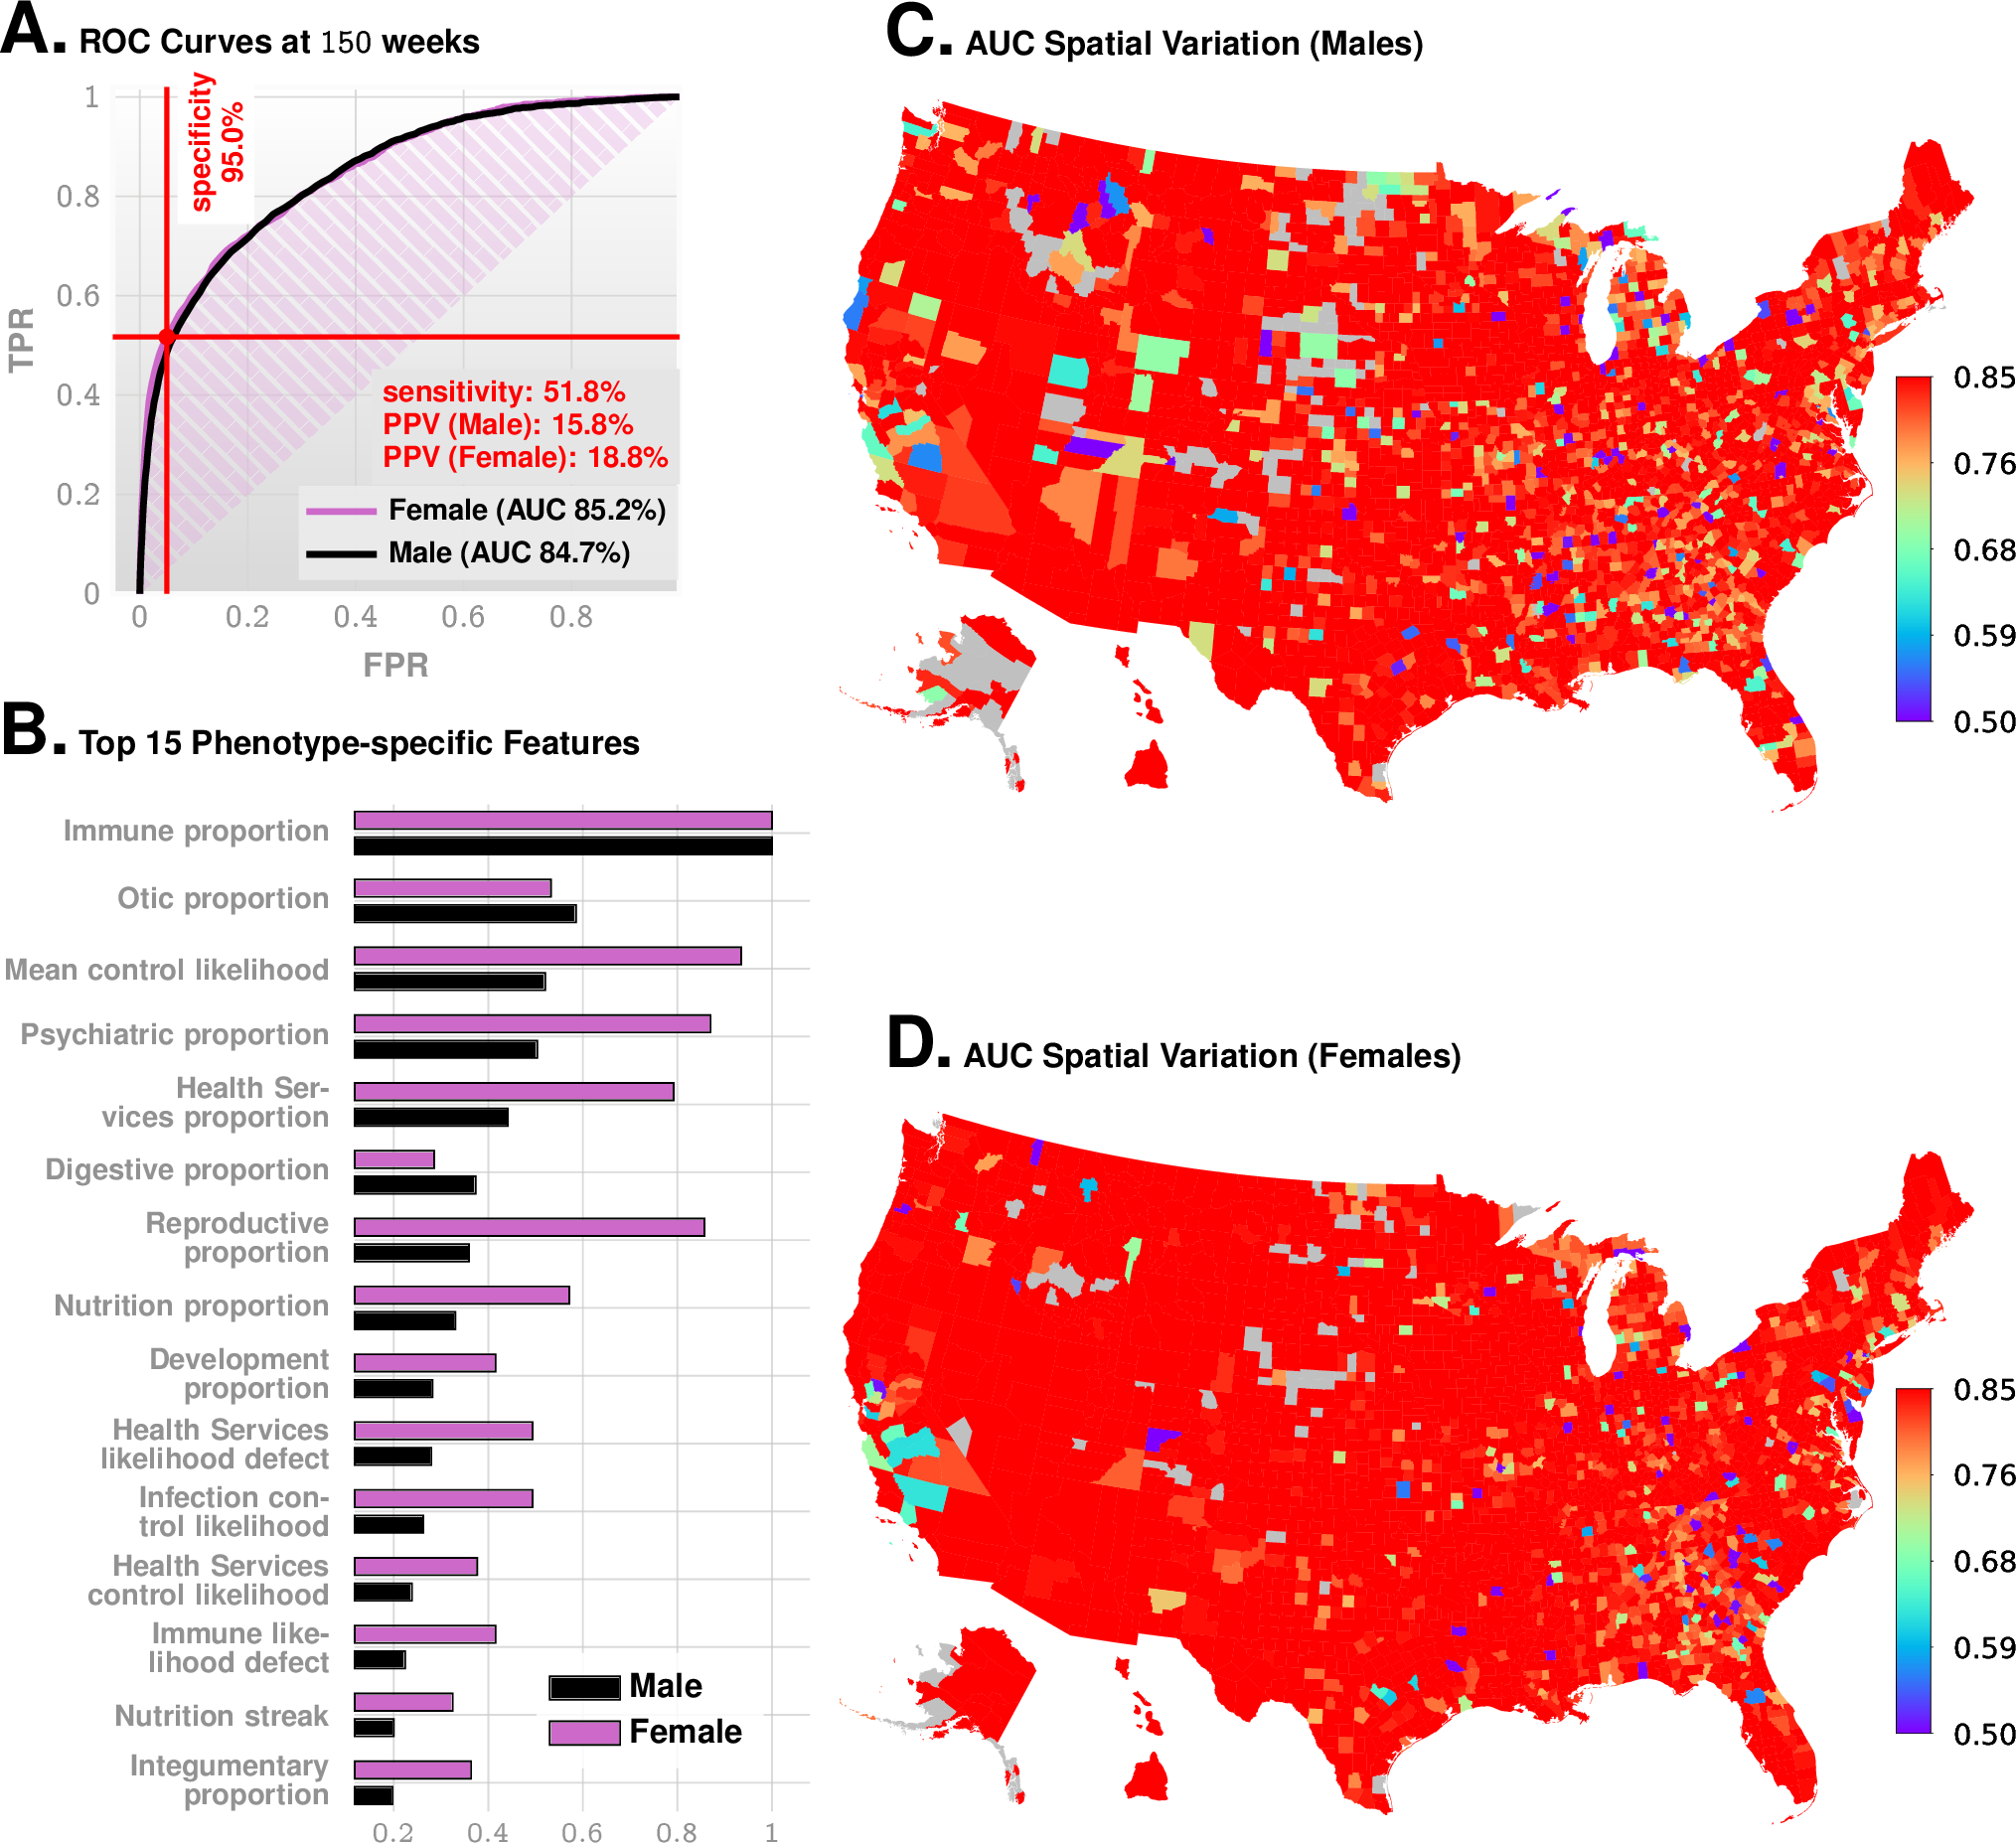
\includegraphics[width=0.85\textwidth]{perfA.pdf}

  \captionN{\textbf{Standalone Predictive Performance of \acor.} Panel A shows the ROC curves for males and females (Truven data shown, UCM is similar, see Fig.~\ref{fig2}a). Panel B shows the feature importance inferred by our prediction pipeline. The detailed description of the features is given in Table~\ref{EXT-tab1}. The most import feature is related to immunologic disorders, and we note that in addition to features related to individual disease categories, we also have the mean control likelihood (rank 3), which may be interpreted as the average likelihood of the diagnostic patterns corresponding to the control category as opposed to the \treatment category. Panels C and D show the spatial variation in the achieved predictive performance at 150 weeks, measured by AUC, for males and females, respectively. Gray areas lack data on either positive or negative cases. These county-specific AUC plots show that the performance of the algorithm has  relatively weak geospatial dependence, which is important in the light of the current uneven distribution of diagnostic resources. Importantly, not all counties have nonzero number of ASD patients; high performance in those counties reflects a small number of false positives with zero false negatives.
  }\label{fig1}
\end{figure*}
% ###########################################################
% ###########################################################
\begin{figure*}[!ht]
  \centering 
  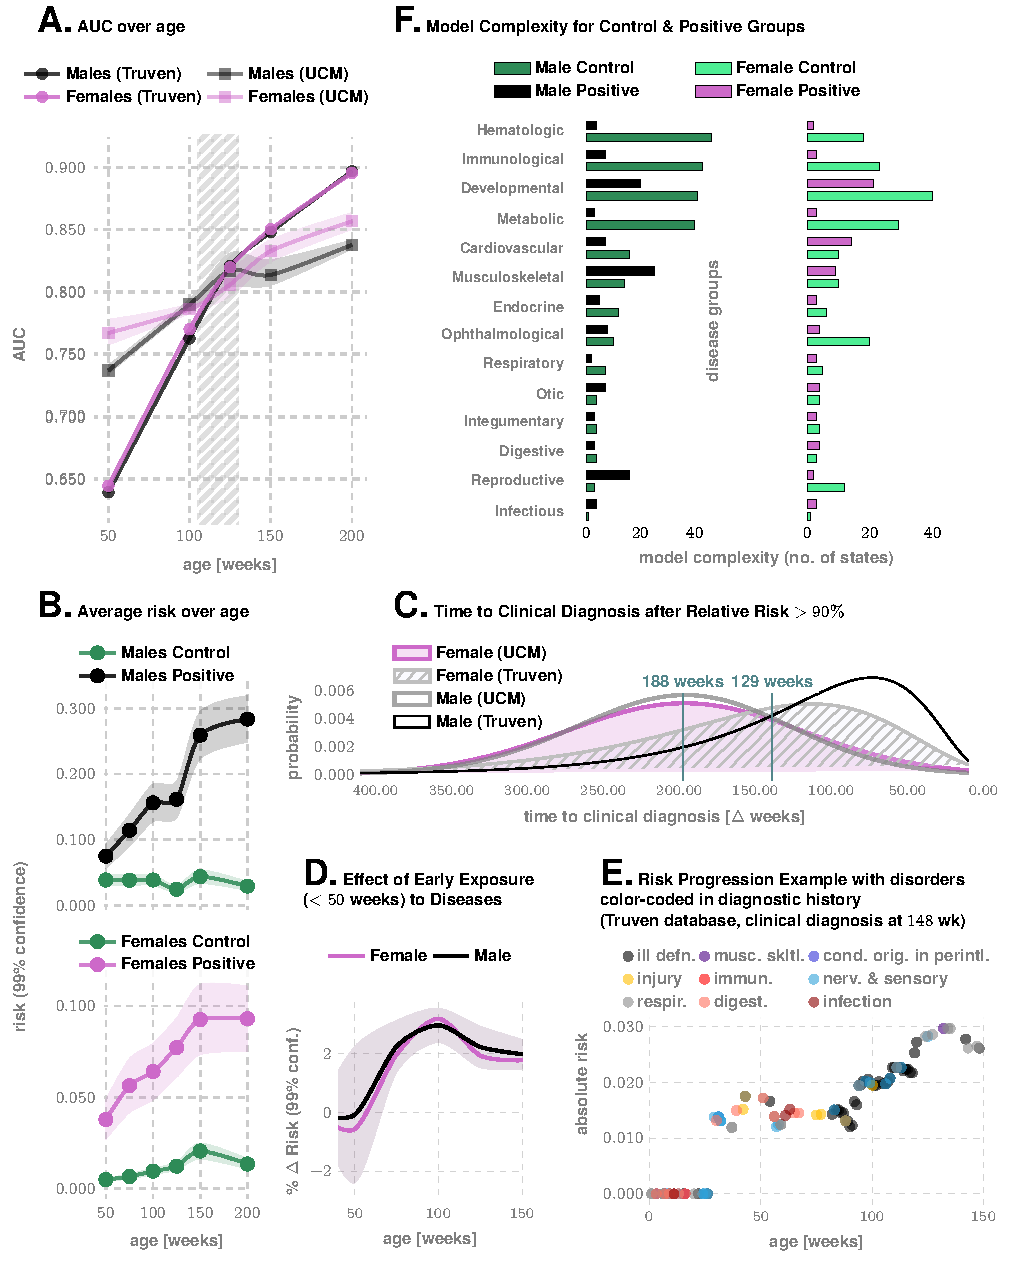
\includegraphics[width=0.85\textwidth]{perfB.pdf}
 
  \captionN{\textbf{More Details on Standalone Predictive Performance of \acor  and Variation of Inferred Risk.} Panel A illustrates AUC achieved as a function of
    patient age, for the Truven and UCM datasets. The shaded area outlines the 2 - 2.5  years of age, and  shows that we achieve $>80\%$ AUC for either sex from shortly after 2 years. Panel B illustrates  how inferred models differ between the control vs. the \treatment cohorts.   Panel C illustrates how the average risk changes with time for the control and the positive cohorts. Note that the risk progressions are somewhat monotonic, and the computed confidence bounds suggest that the odds of a child with low risk upto 100 or 150 weeks of age abruptly shifting to a high risk trajectory is low. Panel D shows the distribution of the prediction horizon: the time to a clinical diagnosis after inferred  relative risk crosses $90\%$. Panel E shows that for each new disease code for a low-risk child, ASD risk increases by approximately $2\%$ for either sex. Panel F illustrates the risk progression of a specific, ultimately autistic male child in the Truven database. Abbreviations in the legend: ill defn. (Symptoms, Signs, And Ill-Defined Conditions),   musc. skltl. (Diseases Of The Musculoskeletal System And Connective Tissue), cond. orig. in perintl. (Certain Conditions Originating In The Perinatal Period), immun. (Endocrine, Nutritional And Metabolic Diseases, And Immunity Disorders), nerv. \& sensory (Diseases Of The Nervous System And Sense Organs), respir. (Respiratory Disorders), and digest. (Digestive Disorders). On average, models get less complex, implying the exposures get more statistically independent.}\label{fig2}
\end{figure*}
% ###########################################################
\begin{figure}[!ht]
  \centering
  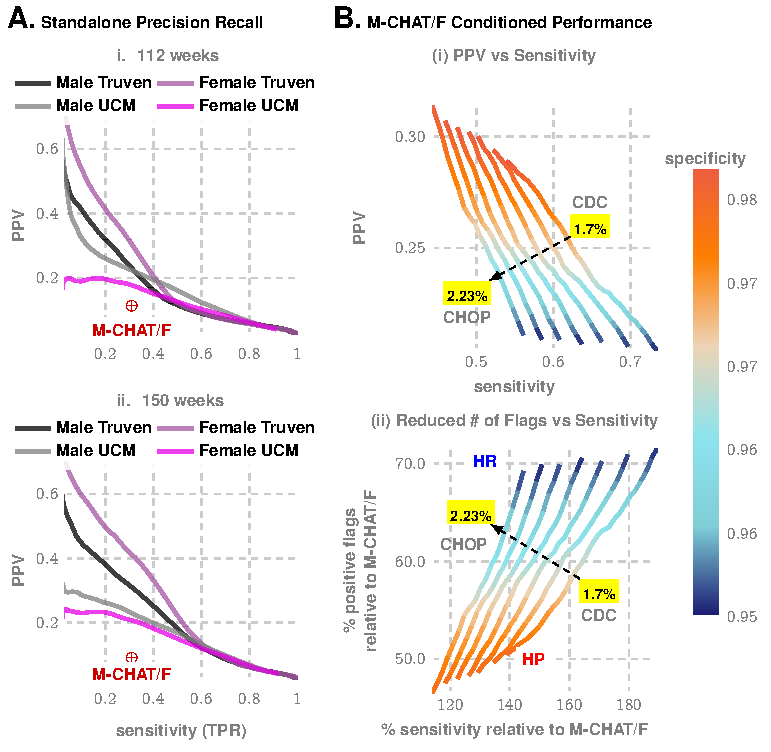
\includegraphics[width=0.75\textwidth]{perfCv.pdf}
 
  \captionN{\textbf{Metrics relevant to clinical practice: PPV vs Sensitivity trade-offs.} Panel A shows the precision/recall curves, $i.e.$,  the trade-off between PPV and sensitivity for \textbf{standalone operation} with \acor. Panel B shows how we can \textbf{boost \acor performance} using population stratification from the distribution of M-CHAT/F scores in the population, as reported by the CHOP study~\cite{pmid31562252}. This is possible because \acor and M-CHAT/F use independent information (co-morbidities vs questionnaire responses).  Note that the population prevalence impacts this optimization, and hence  we have  a distinct  curve for each prevalence value ($1.7\%$ is the CDC estimate, while $2.23\%$ is reported by the CHOP study).  The two extreme operating zones marked as High Precision (HP) and High Recall (HR): if we choose to operate in HR, then we do not reduce the number of positive screens by much, but maximize sensitivity, while by operating in HP, we increase sensitivity by 20-40\% (depending on the prevalence) but double the PPV achieved in current practice. In contrast, when choosing to maximize sensitivity by operating in the HR zone, we only cut down positive flags to about $70\%$ of what we get with M-CHAT/F, but boost sensitivity by $50-90\%$ (Reaching sensitivities over $70\%$). Note in all these zones, we maintain specificity above $95\%$, which is the current state of art, implying that by doubling the PPV, we can halve the number of positive screens currently reported, thus potentially sharply reducing the queues and wait-times. }\label{figprc} 
\end{figure}
% ####################################
\def\RCOL{\rowcolor{teal!40}}
\def\PCOL{Tomato!40}
%#################################### 
\begin{table*}[!ht]
  \centering 
\captionN{Standalone PPV Achieved at 100, 112 and 150 Weeks For Each Dataset and Gender {\bf (M-CHAT/F:  sensitivity=$38.8\%$, specificity=$95\%$, PPV=$14.6\%$ between 16 and  26 months ($\approx$112 weeks))}}\label{EXT-tabssp}

  \vskip .5em

\begin{tabular}{L{.75in}|L{.75in}|L{.75in}|L{.5in}|L{.5in}|L{.75in}}
\hline

weeks&specificity&sensitivity&PPV&gender&dataset\\\hline
100&0.92&0.39&0.14&F&UCM\\\hline
100&0.95&0.39&0.19&M&UCM\\\hline
100&0.93&0.39&0.13&F&Truven\\\hline
100&0.91&0.39&0.10&M&Truven\\\hline
\RCOL 112&0.93&0.39&0.16&F&UCM\\\hline
\RCOL 112&0.95&0.39&0.20&M&UCM\\\hline
\RCOL 112&0.96&0.39&0.22&F&Truven\\\hline
\RCOL 112&0.95&0.39&0.17&M&Truven\\\hline
150&0.94&0.39&0.19&F&UCM\\\hline
150&0.98&0.39&0.34&F&Truven\\\hline
150&0.97&0.39&0.26&M&Truven\\\hline
150&0.97&0.39&0.26&M&UCM\\\hline

  
\end{tabular}%\end{subtable}
\end{table*}  
%#################################### 

\begin{table*}[!ht]
\centering
\captionN{Personalized Operation Conditioned on M-CHAT/F Scores at  26 months}\label{EXT-tabboost}
  \vskip .5em

\begin{tabular} {L{.33in}|L{.33in}|L{.33in}|L{.33in}||L{.35in}|L{.35in}|L{.375in}||L{.375in}|L{.35in}|L{.35in}||L{.6in}}
\hline
\multicolumn{4}{c||}{\cellcolor{lightgray!60}M-CHAT/F Outcome}  & \multicolumn{3}{c||}{\mnp{1.2in}{\vskip .2em global performance (Truven)\vskip .2em  } }&\multicolumn{3}{c||}{\mnp{1.2in}{\vskip .2em global performance\\(UCM)\vskip .2em }} &  \multirow{3}{*}{prevalence$^\star$}\\\cline{0-9}
 0-2  NEG & 3-7  NEG & 3-7  POS & $\geq  8$  POS & \multirow{2}{*}{\mnp{.1in}{speci-ficity}} & \multirow{2}{*}{\mnp{.1in}{sensi-tivity}} &\multirow{2}{*}{PPV}& \multirow{2}{*}{\mnp{.1in}{speci-ficity}} & \multirow{2}{*}{\mnp{.1in}{sensi-tivity}} & \multirow{2}{*}{PPV} & \\\cline{0-3}
\multicolumn{4}{c}{\cellcolor{lightgray} specificity choices}  & & & &&&&\\\hline 

0.2&0.54&0.83&0.98&0.95&0.585&0.209&0.95&0.505&0.186&0.022\\\hline 
0.21&0.53&0.83&0.98&0.95&0.586&0.208&0.95&0.506&0.184&0.022\\\hline 
0.42&0.87&0.98&0.99&\cellcolor{\PCOL}0.98&\cellcolor{\PCOL}0.433\cellcolor{\PCOL}&\cellcolor{\PCOL}0.331&0.98&0.347&0.284&0.022\\\hline 
0.48&0.87&0.97&0.99&\cellcolor{\PCOL}0.98&\cellcolor{\PCOL}0.432&\cellcolor{\PCOL}0.331&0.98&0.355&0.289&0.022\\\hline 
0.38&0.54&0.94&0.98&\cellcolor{\PCOL}0.95&\cellcolor{\PCOL}0.736\cellcolor{\PCOL}&\cellcolor{\PCOL}0.203&0.95&0.628&0.178&0.017\\\hline 
0.3&0.55&0.94&0.98&\cellcolor{\PCOL}0.95&\cellcolor{\PCOL}0.737&\cellcolor{\PCOL}0.203&0.95&0.633&0.179&0.017\\\hline 
0.58&0.96&0.98&0.99&0.98&0.492&0.302&0.98&0.373&0.247&0.017\\\hline 
0.59&0.96&0.98&0.99&0.98&0.491&0.303&0.98&0.372&0.248&0.017\\\hline 
0.46&0.92&0.97&0.99&0.977&0.534&0.291&0.977&0.448&0.256&0.017\\\hline 
0.48&0.92&0.97&0.99&0.978&0.533&0.292&0.978&0.448&0.257&0.017\\\hline 

  
\end{tabular}
\vskip 1em

\flushleft
$^\star$Prevalence reported by CDC is $1.7\%$, while the CHOP study reports a value of $2.23\%$. The results of our optimization depend on the prevalence estimate.
%\end{subtable}
\end{table*}  
%####################################
%###########################################################
\begin{figure*}[!t]
\centering
  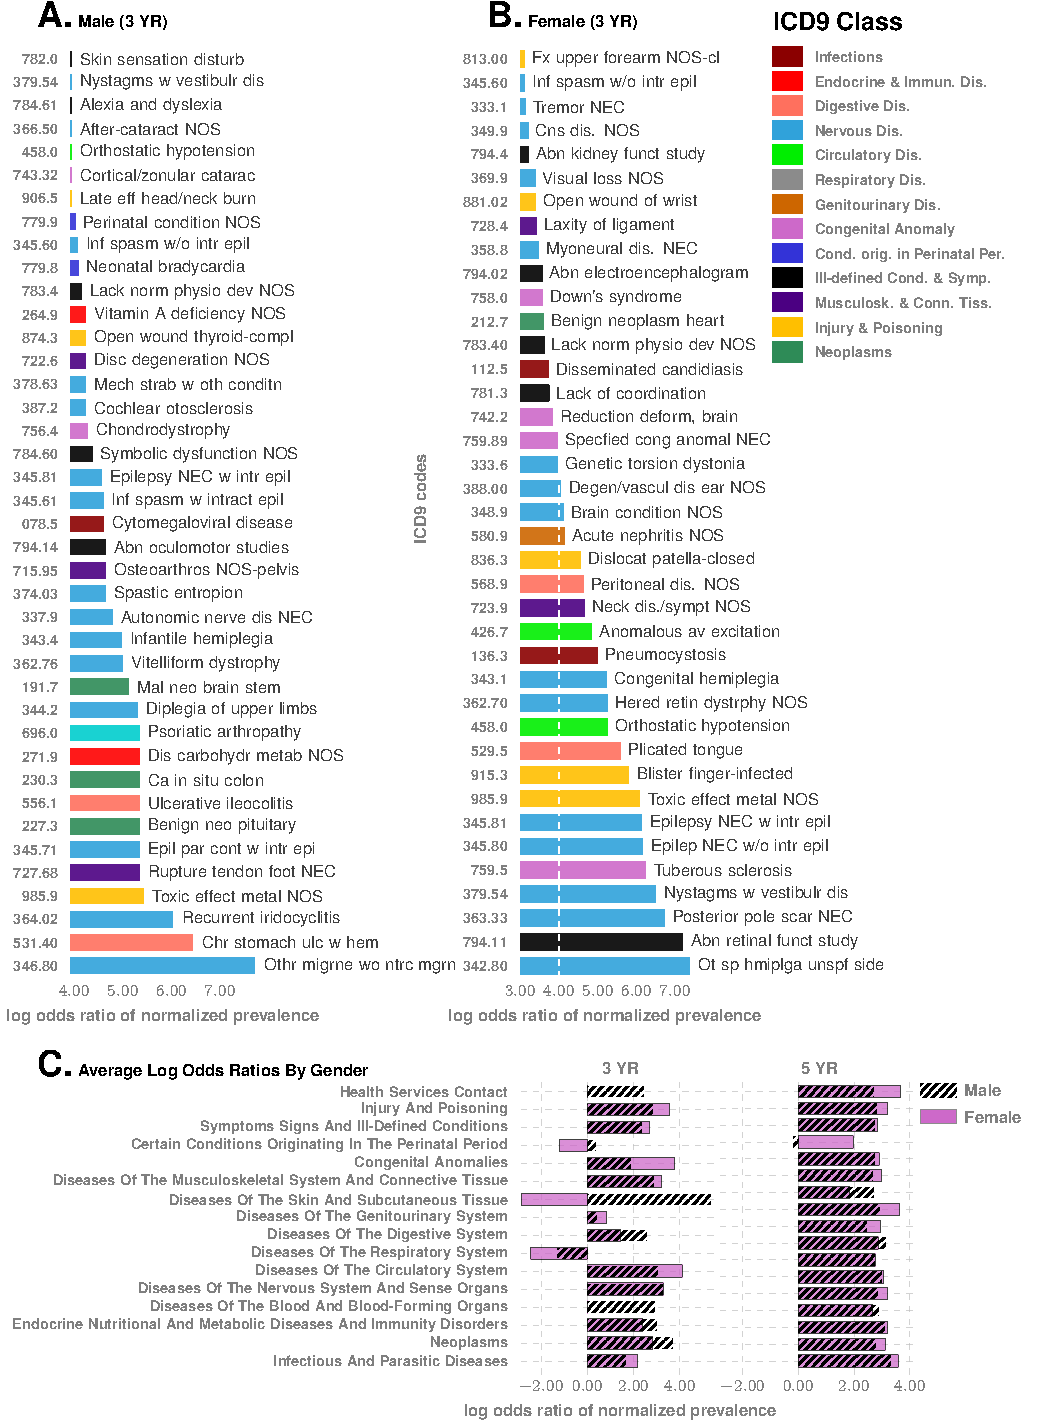
\includegraphics[width=0.9\textwidth]{comorbidA}
 
  \captionN{\textbf{Co-morbidity Patterns} Panel A and B. Difference in occurrence frequencies of diagnostic codes between true positive (TP) and true negative (TN) predictions. The dotted line on panel B shows the  abscissa lower cut-off in Panel A, illustrating the lower prevalence of codes in females. Panel C illustrates log-odds ratios for ICD9 disease categories at different ages. Importantly, the negative associations disappear when we consider older children, consistent with the lack of such reports in the literature which lack studies on very young cohorts. }\label{EXT-fig3}
\end{figure*}


Use of sophisticated analytics to identify children at high risk is a topic of substantial current interest, with independent progress being made by several groups~\cite{hyde2019applications,abbas2020multi,duda2016clinical,duda2014testing,fusaro2014potential,wall2012use,wall2012use2}. Many of these approaches  focus on analyzing questionnaires, with recent efforts demonstrating the use of  automated pattern recognition in video clips of toddler behavior. However, the inclusion of older kids above the age of  $5$ years and  small cohort sizes might limit the immediate clinical adoption of these approaches for universal screening.

Laboratory tests for ASD have also begun to emerge, particularly leveraging detection of abnormal metabolites in plasma~\cite{smith2020metabolomics,howsmon2017classification}, and  salivary poly-omic RNA~\cite{hicks2018validation}. However, as before, inclusion  of older children, limits  applicability in  screening, where we need a decision at $18-24$ months. In addition, such approaches -- while  instrumental in deciphering ASD pathophysiology -- might be too expensive for universal adoption at this time.

In contrast to \acor, the above approaches require additional data or tests. Use of comorbidity patterns derived from past  Electronic Health Records  has been either limited to establishing correlative associations~\cite{doshi2014comorbidity,bishop2018using}, or has substantially underperformed~\cite{lingren2016electronic}(AUC $\leqq 65\%)$ compared to our results.



% \cite{smith2020metabolomics} performed on plasma samples from 708 fasting children, aged 18 to 48 months. 53\% sensitivity (95\% confidence interval [CI], 48\%-57\%) and 91\% specificity (95\% CI, 86\%-94\%).

% \cite{li2018high}predisposition to ASD has been associated with abnormalities of metabolites in folate-dependent one carbon metabolism (FOCM) and transsulfuration (TS). Same data as \cite{howsmon2017classification}

% \cite{hicks2018validation} n=134+238+84, mean age 50 months (4 years). AUC of .88


% \cite{howsmon2017classification} n=208, and age is betwween 3 and 10 years

% Using machine learning and multi-variate statistical analysis to screen for children at higher risk for autism is a topic of substantial interest, with results being reported in several independent research directions. A large number of tehse studies apply analytics to questionaries, or pattren recognition on video clips of toddler behavior. This is distinct from our approach which levergares observed co-morbidities.

% While other ML methods have been attempted, leveraging videos and sophisticated analysis of questionnaires, there is a key difference in the results. All those approaches do not leverage comorbidity. In some sense such approaches model the physician, no new insight is often possible fro such approaches. We other other hand model the disease processes and it footprint in different functions systems that manifest as subtle difference in comorbidity patterns. Thus, we model the disease more directly, and there is clear opportunity to gaining new insight into the pathophysiology of autism.

% \cite{doshi2014comorbidity}: small cohort, age 0-15, only correlation shown.

% \cite{lingren2016electronic}: n152, auc=65\%

% \cite{pmid27185194}: no autism

% \cite{abbas2020multi}:n=375, 18-72 months, auc$>90\%$ questionnaire, video and clinician inputs

% \cite{tariq2018mobile}: Mean age 4years $\pm$ 2 yrs , n=116, video, auc=92\%, blinded nonexpert raters from 3-minute home videos of children with and without ASD 

% \cite{duda2016clinical}, mean age 5.8 years, Children 16 months–17 years (N = 222)
% were screened during their first visit in a developmental-
% behavioral pediatric clinic.

% \cite{duda2014testing}, applies to ADOS, significantly correlated with the ADOS-G (r=-0.814) and ADOS-2 (r=-0.779) and exhibited $>97\%$ sensitivity and $>77\%$ specificity in comparison to both ADOS algorithm scores. The cohort studied was 76.8\% male, 18.5\% female and 4.7\% unknown gender, and the average age at testing was 6.21 years (±4.25 years).


% \cite{fusaro2014potential}, n=100, videos and non-clinical raters, results also demonstrate the potential for video-based detection of autism in short, unstructured home videos. classification accuracy was 96.8\%, with 94.1\% sensitivity and 100\% specificity, 

% \cite{wall2012use} questionnaire, ADOS, mostly older kids with average age around 5 years. high performance

% \cite{wall2012use2} ADOS, targets behavior between ages of 4 and 5, questionnaire, high performance




\section*{Materials \& Methods}
% ##########################################
% ##########################################
% ###########################################################
%\subsection*{Source of Electronic Patient Records}

We view the task of predicting  ASD diagnoses   as a binary classification problem: sequences of diagnostic codes are classified into positive and control categories, where ``positive'' refers to children eventually diagnosed with ASD, as indicated by the presence of a clinical diagnosis (ICD9 code 299.X) in their medical records. Of the two independent sources of clinical incidence data used in this study,  the primary source used to train our predictive pipeline  is the Truven Health Analytics MarketScan\textsuperscript{\textregistered} Commercial Claims and Encounters Database for the years 2003 to 2012~\cite{hansen2017truven} (referred to  as the Truven dataset). This US national database merges  data contributed by over 150 insurance carriers and large self-insurance companies,  and comprises over  4.6 billion inpatient and outpatient service claims and  almost six billion diagnosis codes. We extracted histories of patients within the age of $0-6$ years, and excluded  patients for whom:  1) At least one code of any available phenotypes is present, 2) The first and last available record for a patient are  at least 15 weeks apart. These exclusion criteria ensure that we are not considering patients who have too few observations. Additionally, during validation runs,  we restricted the control set to patients observable in the databases to those whose last record is not before the first 150 weeks of life. Characteristics of excluded patients is shown in Table~\ref{tab2}. We trained with over  30M diagnostic records (16,649,548 for males and  14,318,303  for females with 9,835 unique  codes).

While the Truven database is used for both training and out-of-sample cross-validation with held-back  data, our second independent dataset  comprising de-identified diagnostic records for children treated at the University of Chicago Medical Center between the years of 2006 to 2018 (the UCM dataset) aids in further cross-validation. We considered children between the ages of $0-6$ years, and  applied the same exclusion criteria as the Truven dataset.  The  number of  patients used from the two databases is shown in Table~\ref{tab2}. Our datasets are consistent with documented ASD prevalence and median diagnostic age (3 years in the claims database  versus 3 years 10 months to 4 years  in US~\cite{pmid29701730}) with no significant geospatial prevalence variation (See SI-Fig.~\ref{SI-figocc}).

%and reveal that  infections and immunological disorders have differential representation in the \treatment and control groups (Fig.~\ref{EXT-fig0}C).
The  median diagnosis age is  just over  3 years in the claims database  versus 3 years 10 months to 4 years  in US~\cite{pmid29701730}. %Cohort details are given in Table~\ref{tab2} and discussed in Methods. For the positive cohort, we only consider diagnostic history up to the first ASD code.

% XXXXXX

% XXXXX two codes
% XXX what if children do not have ehr data

% is there a minumu number of codes used

% duisdae prevalence in the two databases

% comment pon filling with zeroes

The significant diversity of diagnostic codes (6,089 distinct ICD-9 codes and 11,522 distinct ICD-10 codes in total in the two datasets), along with the sparsity of codes per sequence and the need to make good predictions as early as possible,  makes this a difficult learning problem, and standard deep learning approaches do not yield sufficiently high predictive performance or statistical power (See Supp. Fig.~\ref{SI-EXT-figcompwsoa}). Thus, we proceed by  partitioning the  disease spectrum into $17 $ broad categories, $e.g.$ infectious diseases, immunologic disorders, endocrinal disorders etc. Each patient is then represented by $17$ distinct time series, each  tracking an individual disease category. At the population level, these disease-specific sparse stochastic time series are  compressed into specialized Markov models (separately for the control and the treatment cohorts) to identify  the distinctive patterns  pertaining to elevated ASD risk. Each of these inferred models in a Probabilistic Finite State Automaton (PFSA). See Supplementary Text Section~\ref{SI-sec:PFSA} for details on PFSA inference.  

We use a novel approach to evaluate subtle deviations in stochastic observations known as the sequence likelihood defect (SLD), to  quantify similarity of observed time-series of diagnostic events to the control vs the \treatment cohorts for individual patients. This novel stochastic inference approach provides  significant boost to the overall performance of our predictors; with only state of the art machine learning  the predictive performance is significantly worse (See Supplementary Text Sections~\ref{SI-sec:pipelinevar} and \ref{SI-sec:offtheshelf}, as well as reported performance in the literature for predicting ASD risk from EHR data with standard algorithms~\cite{lingren2016electronic}).

% To provide a brief outline of the SLD computation, we note that for each patient, the past  medical history is a sequence $(t_1,x_1),\cdots,(t_m,x_m)$, where $t_i$ are timestamps and $x_i$ are ICD codes diagnosed at time $t_i$.  We map individual patient history to a three-alphabet categorical time series $z^k$ corresponding to the disease category $k$,  as follows. For each week $i$, we have: 
% \cgather{\label{eq1}
%   z^k_i =  \left \{ \begin{array}{ll}
%                       0 & \textrm{if no diagnosis codes  in week } i\\
%                       1 & \textrm{if there exists a diagnosis of category $k$ in week } i\\
%                       2 & \textrm{otherwise}
%                     \end{array} \right.
%                 }%
% The time-series $z^k$ is terminated at a particular week if the patient is diagnosed with ASD the week after. Thus for patients in the control cohort, the length of the mapped trinary series is limited by the time for which the individual is observed within the  2003 -- 2012 span of our database. In contrast, for patients in  the \treatment cohort, the length of the mapped series reflect the time to the first ASD diagnosis. Patients do not necessarily enter the database at birth, and we prefix each series with 0s to  approximately synchronize observations to age in weeks. %Each patient is now represented by $17$ mapped trinary series.

% We use  the mapped series, stratified by  sex, disease-category, and ASD diagnosis-status  to infer specialized HMMs. We model the \treatment and the control cohorts for each sex, and in  each disease category separately, ending up with a total of $68$ HMMs at the population level ($17$ categories, $2$ sexes, $2$ cohort-types: \treatment and control, SI-Fig.~\ref{SI-EXT-autgrid} in the supplementary text provides some examples). Each of these inferred models is  a Probabilistic Finite State Automata (PFSA);  a directed graph with probability-weighted edges, and acts as an optimal generator of the  stochastic process driving the  sequential appearance of the three letters (as defined by Eq.~\eqref{eq1})  corresponding to each sex, disease category, and cohort-type (See Section~\ref{SI-sec:PFSA} in the Supplementary text for  background on PFSA inference). 

We briefly outline the SLD computation: To reliably infer the cohort-type of a new patient, $i.e$, the likelihood of a diagnostic sequnce being generated by the corresponding cohort model, we generalize the notion of Kullbeck-Leibler (KL) divergence~\cite{Cover,kullback1951} between probability distributions to a divergence $\mathcal{D}_{\textrm{KL}}(G \vert \vert H)$ between ergodic stationary categorical stochastic processes~\cite{doob1953stochastic} $G,H$ as:
\cgather{
  \mathcal{D}_{\textrm{KL}}(G \vert \vert H) = \lim_{n\rightarrow \infty} \frac{1}{n}  \sum_{x:|x| = n}p_G(x)\log\frac{p_G(x)}{p_H(x)}  }%
where $\vert x\vert $ is the sequence length, and $p_G(x) ,p_H(x) $ are the probabilities of sequence $x$ being generated by the processes $G,H$ respectively. Defining the  log-likelihood of  $x$ being generated by a process $G$ as:
\cgather{
  L(x,G)= -\frac{1}{\vert x\vert}\log p_G(x) 
}%
The cohort-type for an observed sequence $x$ | which is actually generated by the hidden process $G$ | can be formally inferred from observations based on the following provable relationships (See Suppl. text Section~\ref{SI-sec:PFSA}, Theorem 6 and 7):
\begin{subequations}\label{eqR}\cgather{
    \lim_{\vert x \vert \rightarrow \infty}L(x,G) = \mathcal{H}(G)   \\
    \lim_{\vert x \vert \rightarrow \infty } L(x,H)  =\mathcal{H}(G) +  \mathcal{D}_{\textrm{KL}}(G \vert \vert H)   
  }\end{subequations}%
where  $\mathcal{H}(\cdot)$ is the entropy rate of a process~\cite{Cover}. Importantly, Eq.~\eqref{eqR} shows that the computed likelihood has an additional non-negative contribution from the divergence term when we choose the incorrect generative process.  Thus, if a  patient is eventually going to be diagnosed with ASD, then we expect that the disease-specific mapped series corresponding to  her diagnostic history be modeled by the corresponding model in the \treatment cohort. Denoting the model  corresponding to disease category $j$ for \treatment and control cohorts as $G^{j}_+,G^{j}_0$ respectively, we can compute the sequence likelihood defect (SLD, $\Delta^j$) as:
\cgather{
  \Delta^j \triangleq L(G^{j}_0,x) - L(G^{j}_+,x) \rightarrow \mathcal{D}_{\textrm{KL}}(G^{j}_0 \vert \vert G^{j}_+) \label{eq6}
}%
With  the inferred   models and  the individual diagnostic history, we  estimate the SLD measure on the  right-hand side of Eqn.~\eqref{eq6}. The higher this likelihood defect, the higher  the similarity of diagnosis history to that of children with autism.
                

In addition to the category specific Markov models, we use a range of engineered features that reflect various aspects of the diagnostic histories, including the porportion of weeks in which a diagnostic code is generated, the maximum length of consecutive weeks with codes, the maximum length of weeks with no codes (See Tab.~\ref{EXT-tab1} for complete description), resulting in a total of $165$ different features that are evaluated for each patient. With these inferred patterns included as features,  we train a second level predictor that learns to map   individual patients  to the control or the \treatment groups based on their  similarity  to the identified  Markov models of category-specific diagnostic histories, and the other engineered features (See Section~\ref{SI-sec:mathdetails} on detailed mathematical details  in Supplementary  text).
%

Since we need to infer the Markov models prior to the calculation of the likelihood defects, we need two training sets: one that is used to infer the models, and one that subsequently trains the final classifier  with features  derived  from the inferred models along with other engineered features. Thus, the analysis proceeds by first carrying out a random 3-way split of the set of unique patients (in the Truven dataset) into \textit{Markov model inference} ($25\%$), \textit{classifier training} ($25\%$) and \textit{test} ($50\%$) sets. The approximate sample sizes of the three sets are as follows: $\approx 700K$ for each of  the training sets, and $\approx 1.5M$ for the test set. The features used in our pipeline may be ranked in order of their relative importance (See Fig.~\ref{fig1}B for the top 15 features), by
estimating the loss in performance when dropped out of the analysis. We verified that different random splits do not adversely affect performance. The UCM dataset in its entirety is used as a test set, with no retraining of the pipeline.

%This novel two step learning algorithm outperforms standard tools, and achieves  stable performance across datasets. 
%####################
% \subsection*{Time-series Modeling of  Diagnostic History}
% Individual diagnostic histories  can have long-term memory~\cite{ltgranger80}, implying that the order, frequency, and comorbid interactions between diseases are   important for assessing the future risk of our target phenotype. 
% We analyze  patient-specific  diagnostic code sequences by first  representing the medical history of each patient as a set of stochastic categorical time-series | one each for a specific group of related disorders |  followed by the inference of stochastic models  for  these individual data streams. These inferred generators are from a special class of  Hidden Markov Models (HMMs), referred to as Probabilistic Finite State Automata (PFSA)~\cite{CL12g}. The inference algorithm we use is distinct from classical HMM learning, and has important advantages related to its ability to infer structure, and its sample complexity (See Supplementary text, Section~\ref{SI-sec:PFSA}). We infer a separate class of models for the \treatment and control cohorts, and then the problem reduces to determining the probability that the short diagnostic history from a  new  patient arises from the \treatment as opposed to the control category of the inferred models. 
% %####################
% \subsection*{Step 1: Partitioning The Human Disease Spectrum}
% We begin by partitioning the human disease spectrum into  $17$ non-overlapping  categories,  as shown in Table~\ref{EXT-tab0}. Each category is defined by a set of diagnostic codes from the International Classification of Diseases, Ninth Revision (ICD9) (See Table~\ref{EXT-tab0} in the main text  and Table SI-\ref{SI-tab0} in the Supplementary text for description of  the categories used in this study).
% For this study, we considered $9,835$ distinct ICD9 codes (and their ICD10 General Equivalence Mappings (GEMS)~\cite{GEMS} equivalents). We came across 6,089 distinct ICD-9 codes and 11,522 distinct ICD-10 codes in total in the two datasets we analyzed. Transforming the diagnostic histories to report only the broad categories   reduces the number of distinct codes that the pipeline needs to handle, thus improving statistical  power.  %The trade-offs for this increased power consist of 1) the loss of distinction between disorders in the same category, and  2) some inherent subjectivity in determining the constituent ICD9 codes that define each category, $e.g.$ an ear infection may be classified either an otic disease or an infectious one.
% % 
% Our categories largely align with the top-level ICD9 categories, with small 
% adjustments, $e.g.$ bringing all infections under one category irrespective of the pathogen or the target organ.
% We do not pre-select the phenotypes; we want our algorithm to seek out the important patterns without any manual curation of the input data. The limitation of the set of phenotypes to $9835$ unique codes arises from excluding patients from the database who have very few and rare codes that will skew the statistical estimates. As shown in Table~\ref{tab2}, we exclude a very small number of patients, and who have  very short diagnostic histories with a very small number of codes.

% % Next, we process raw diagnostic histories to  report only the categories. 
% For each patient, the past  medical history is a sequence $(t_1,x_1),\cdots,(t_m,x_m)$, where $t_i$ are timestamps and $x_i$ are ICD9 codes diagnosed at time $t_i$.  We map individual patient history to a three-alphabet categorical time series $z^k$ corresponding to the disease category $k$,  as follows. For each week $i$, we have: 
% \cgather{\label{eq1}
%   z^k_i =  \left \{ \begin{array}{ll}
%                       0 & \textrm{if no diagnosis codes  in week } i\\
%                       1 & \textrm{if there exists a diagnosis of category $k$ in week } i\\
%                       2 & \textrm{otherwise}
%                     \end{array} \right.
%                 }\noindent
%                 The time-series $z^k$ is terminated at a particular week if the patient is diagnosed with ASD the week after. Thus for patients in the control cohort, the length of the mapped trinary series is limited by the time for which the individual is observed within the  2003 -- 2012 span of our database. In contrast, for patients in  the \treatment cohort, the length of the mapped series reflect the time to the first ASD diagnosis. Patients do not necessarily enter the database at birth, and we prefix each series with 0s to  approximately synchronize observations to age in weeks. Each patient is now represented by $17$ mapped trinary series.
% %####################
% \subsection*{Step 2: Model Inference \& The Sequence Likelihood Defect}
% The mapped series, stratified by  sex, disease-category, and ASD diagnosis-status are considered to be independent sample paths, and we want to explicitly model these systems as specialized HMMs (PFSAs). We model the \treatment and the control cohorts for each sex, and in  each disease category separately, ending up with a total of $68$ HMMs at the population level ($17$ categories, $2$ sexes, $2$ cohort-types: \treatment and control, SI-Fig.~\ref{SI-EXT-autgrid} in the supplementary text provides some examples). Each of these inferred models is  a PFSA;  a directed graph with probability-weighted edges, and acts as an optimal generator of the  stochastic process driving the  sequential appearance of the three letters (as defined by Eq.~\eqref{eq1})  corresponding to each sex, disease category, and cohort-type (See Section~\ref{SI-sec:PFSA} in the Supplementary text for  background on PFSA inference). 

% To reliably infer the cohort-type of a new patient, $i.e$, the likelihood of a diagnostic sequnce being generated by the corresponding cohort model, we generalize the notion of Kullbeck-Leibler (KL) divergence~\cite{Cover,kullback1951} between probability distributions to a divergence $\mathcal{D}_{\textrm{KL}}(G \vert \vert H)$ between ergodic stationary categorical stochastic processes~\cite{doob1953stochastic} $G,H$ as:
% \cgather{
%   \mathcal{D}_{\textrm{KL}}(G \vert \vert H) = \lim_{n\rightarrow \infty} \frac{1}{n}  \sum_{x:|x| = n}p_G(x)\log\frac{p_G(x)}{p_H(x)}  }%
% where $\vert x\vert $ is the sequence length, and $p_G(x) ,p_H(x) $ are the probabilities of sequence $x$ being generated by the processes $G,H$ respectively. Defining the  log-likelihood of  $x$ being generated by a process $G$ as :
% \cgather{
%   L(x,G)= -\frac{1}{\vert x\vert}\log p_G(x) 
% }%
% The cohort-type for an observed sequence $x$ | which is actually generated by the hidden process $G$ | can be formally inferred from observations based on the following provable relationships (See Suppl. text Section~\ref{SI-sec:PFSA}, Theorem 6 and 7):
% \begin{subequations}\label{eqR}\cgather{
%     \lim_{\vert x \vert \rightarrow \infty}L(x,G) = \mathcal{H}(G)   \\
%     \lim_{\vert x \vert \rightarrow \infty } L(x,H)  =\mathcal{H}(G) +  \mathcal{D}_{\textrm{KL}}(G \vert \vert H)   
%   }\end{subequations}%
% where  $\mathcal{H}(\cdot)$ is the entropy rate of a process~\cite{Cover}. Importantly, Eq.~\eqref{eqR} shows that the computed likelihood has an additional non-negative contribution from the divergence term when we choose the incorrect generative process.  Thus, if a  patient is eventually going to be diagnosed with ASD, then we expect that the disease-specific mapped series corresponding to  her diagnostic history be modeled by the PFSA in the \treatment cohort. Denoting the PFSA corresponding to disease category $j$ for \treatment and control cohorts as $G^{j}_+,G^{j}_0$ respectively, we can compute the \textit{sequence likelihood defect} (SLD, $\Delta^j$) as:
% \cgather{
%   \Delta^j \triangleq L(G^{j}_0,x) - L(G^{j}_+,x) \rightarrow \mathcal{D}_{\textrm{KL}}(G^{j}_0 \vert \vert G^{j}_+) \label{eq6}
% }%
% With  the inferred  PFSA  models and  the individual diagnostic history, we  estimate the SLD measure on the  right-hand side of Eqn.~\eqref{eq6}. The higher this likelihood defect, the higher  the similarity of diagnosis history to that of children with autism.
% %####################
% \subsection*{Step 3: Risk Estimation Pipeline With Semi-supervised \& Supervised Learning Modules}
% The risk estimation pipeline operates on patient specific information limited to the sex and available  diagnostic history from birth, and produces an estimate of the relative risk of ASD diagnosis at a specific age, with an associated  confidence value. To learn the parameters and associated model structures of  this pipeline, we transform the patient specific data to a set of engineered features, and the feature vectors realized on the
% \treatment and control sets are  used to train a gradient-boosting classifier~\cite{gbm02}. The complete list of $165$ features used  is provided in Table~\ref{EXT-tab1}.

% We need two training sets: one to infer the models, and one to  train the classifier  with features  derived  from the inferred models. Thus, we do a random 3-way split of the set of unique patients into \textit{feature-engineering} ($25\%$), \textit{training} ($25\%$) and \textit{test} ($50\%$) sets. We use the feature-engineering set of ids first to infer our PFSA models \textit{(unsupervised model inference in each category)}, which then allows us to train the gradient-boosting classifier using the training set and PFSA models \textit{(classical supervised learning)}, and we finally execute  out-of-sample validation on the test set. Fig.~\ref{fig1}B shows the top $15$ features  ranked in order of their relative importance (relative loss in performance when dropped out of the analysis). 
%####################
%\subsection*{Calculating Relative Risk}
Our pipeline maps medical histories to a   raw indicator of 
risk. Ultimately, to make crisp predictions, we must choose  a decision threshold for this raw score. % Conceptually identical to the notion of Type 1 and Type 2 errors in classical statistical analyses, the choice of a threshold trades off false positives (Type 1 error) for false negatives (Type 2 error): choosing a small threshold  results in predicting a larger fraction of future diagnoses correctly, $i.e.$ have a high true positive rate (TPR), while simultaneously suffering from a higher false positive rate (FPR), and vice versa. Therefore, a choice of a specific decision threshold   reflects a choice of the maximum FPR and minimum TPR, and is   driven by the application at hand.
In this study, we base our analysis on maximizing the $F_1$-score, defined as the harmonic mean of sensitivity and specificity, to make a   balanced trade-off between Type 1 and Type 2 errors (See Supplementary text, Section~\ref{SI-sec:F1}). The \textit{relative risk} is then defined as the ratio of the raw  risk to the  decision threshold, and a value  $>1$  predicts a future ASD diagnosis. Our two step learning algorithm outperforms standard tools, and achieves  stable performance across datasets strictly superior to documented M-CHAT/F.
%####################
%\subsection*{Boosting Performance Via Leveraging Population Stratification Induced By Existing Tests}
%


The independence of our approach from questionnaire based screening implies that we can further boost our performance by conditioning choice of the sensitivity/specificity trade-offs on individual M-CHAT/F scores. In particular, we leverage the population stratification induced by M-CHAT/F to improve combined performance. Here a combination of \acor with M-Chat/F refers to the conditional choice of the sensitivity/specificity trade-offs for \acor in each sub-population such that the overall performance is maximized. %optimized with respect to whether we wish to maximize the PPV or the sensitivity at a specified minimum level of specificity.

Assume that there are $m$ sub-populations such that: the sensitivities, specificities achieved, and the prevalences in each sub-population are given by $s_i,c_i$ and $\rho_i$ respectively, with $ i \in \{1,\cdots, m\}$. Let $\beta_i$ be the relative size of each sub-population. Then, we have (See Supplementary text, Section~\ref{SI-subsec:4D}):
\begin{subequations}\label{eqscpop}
  \cgather{
    s= \sum_{i=1}^m s_i \gamma_i  \\
    c= \sum_{i=1}^m c_i \gamma_i' %\\PPV = \frac{s}{s+(1-c)(\frac{1}{\rho} -1)}
    \intertext{
      where we have denoted:
    }
    \gamma_i = \beta_i \frac{\rho_i }{\rho}, \textrm{ and }  \gamma_i'= \beta_i \frac{1-\rho_i}{1-\rho}
  }%
\end{subequations}%
and $s,c,\rho$ are the overall sensitivity, specificity, and prevalence. Knowing the values of $\gamma_i, \gamma_i'$, we can carry out an $m$-dimensional search to identify the feasible choices of $s_i,c_i$ pairs for each $i$, such that some global constraint is satisfied, $e.g.$ minimum values of specificity, sensitivity, and PPV.
We consider  $4$ sub-populations defined by M-CHAT/F score brackets~\cite{pmid31562252}, and if the screen result is considered a positive (high risk, indicating the need for a full diagnostic evaluation) or a negative, $i.e. $, low risk: 1) score   $\leq 2$  screening ASD negative, 2) score $[3-7]$ screening ASD negative on follow-up, 3) score  $[3-7]$ and  screening ASD positive on follow-up, and 4) score  $\geq 8$,  screening ASD positive. (See SI-Table~\ref{SI-EXT-tabCHOP}). The ``follow-up'' in the context of M-CHAT/F refers to the re-evaluation of responses by qualified personnel. We use published data from the CHOP study~\cite{pmid31562252} on the relative sizes and the prevalence statistics in these sub-populations to   compute the feasible conditional choices of our  operating point  to vastly supersede standalone M-CHAT/F performance. The CHOP study  is the only large-scale study of M-CHAT/F we are aware of with sufficient follow-up after the age of four years to provide a reasonable degree of confidence in the sensitivity of M-CHAT/F.

% XXXXXXX

Two limiting operating conditions are  of special interest in this optimization scheme, 1) where we maximize PPV under some minimum specificity and sensitivity (denoted as  the High Precision or the HP operating point), and 2) where we maximize sensitivity under some minimum PPV and specificity (denoted as the High Recall or the HR  operating point). Taking these minimum values of specificity, sensitivity, and PPV to be those reported for  M-CHAT/F, we identify the set feasible set of conditional choices in a four-dimensional decision space  that would  significantly outperform M-CHAT/F in universal screening. The results are shown in Fig.~\ref{figprc}B.

We carried out a battery of tests to ensure that our results are not significantly impacted by class imbalance (since our control cohort is orders of magnitude larger) or systematic coding errors, $e.g.$, we verified that restricting the \treatment cohort to children with at least two  distinct ASD diagnostic codes in their medical histories instead of one, has little impact on  out-of-sample predictive performance (SI-Fig.~\ref{SI-EXT-figcompsi}B). 


% ####################

\section*{Results}
We measure our performance using several standard metrics including the AUC, sensitivity, specificity and the PPV. For the prediction of the eventual ASD  status, we achieve an out-of-sample AUC of $82.3\%$ and  $82.5\%$ for males and females respectively at $125$ weeks for the Truven dataset. In the UCM dataset, our performance is comparable: $83.1\%$ and $81.3\%$ for males and females respectively (Fig.~\ref{fig1} and \ref{fig2}).  Our AUC is shown to improve approximately  linearly  with patient age: Fig.~\ref{fig2}A illustrates that the  AUC  reaches 90\%  in the Truven dataset at the age of four.

Recall, that the UCM dataset is used purely for validation, and good  performance on these independent datasets lends strong evidence for our claims. Furthermore, applicability in new datasets \textit{without local re-training} makes it readily  deployable in clinical settings.

%What are the inferred patterns that  elevate risk?  
Enumerating the top $15$ predictive features (Fig.~\ref{fig1}B), ranked  according to their automatically inferred weights  (the feature ``importances''), we found that while infections and immunologic disorders are the most predictive, there is significant effect from all the $17$ disease categories. Thus, the  co-morbid indicators are  distributed across the disease spectrum, and no single  disorder is uniquely implicated (See also Fig.~\ref{fig2}F). Importantly, predictability is relatively agnostic to the number of local cases across US counties (Fig.~\ref{fig1}C-D) which is important in light of the current uneven distribution of  diagnostic resources~\cite{gordon2016whittling,althouse2006pediatric} across states and regions.
 
Unlike individual predictions which only become relevant over 2 years, the average risk over the populations is clearly different  from around the  first birthday (Fig.~\ref{fig2}B), with the risk for the  \treatment cohort rapidly rising. Also, we see a saturation of the risk after $\approx 3$ years, which corresponds to the median diagnosis age in the database. Thus, if a child is not diagnosed up to that age, then the  risk  falls, since the probability of a diagnosis in the population starts to go down after this age. While average discrimination is not useful for individual patients, these reveal important clues as to how the  risk evolves over time. Additionally, while  each  new diagnostic code within the first year of life  increases the risk burden by approximately $2\%$ irrespective of sex (Fig.~\ref{fig2}D), distinct  categories modulate the risk differently, $e.g.$, for a single random patient  illustrated in Fig.~\ref{fig2}F infections and immunological disorders dominate early, while  diseases of the nervous system and sensory organs, as well as ill-defined symptoms,  dominate the latter period.

Given these results, it is important to ask how much earlier can we trigger an intervention? On average,  the first time the relative risk (risk divided by the decision threshold set to maximize F1-score, see Methods) crosses the $90\%$ threshold precedes  diagnosis by  $\approx 188$ weeks in the Truven dataset, and $\approx 129$ weeks in the UCM dataset. This does not mean that we are   leading a possible clinical diagnosis by over $2$ years; a significant portion of this delay arises from families waiting in queue for diagnostic evaluations. Nevertheless, since delays are rarely greater than   one year~\cite{gordon2016whittling},  we are still likely to produce valid red flags significantly earlier than the current practice.%, potentially cutting down the mean diagnostic age by over $1.5$ years.

Our approach produces a strictly superior PPV (exceeding M-CHAT/F PPV by at  least $14\%$ (14.1-33.6\%) when sensitivity and specificity are held at comparable values (approx. $38\%$ and $95\%$) around the age of 26 months ($\approx 112$ weeks). Fig.~\ref{figprc}A and Table~\ref{EXT-tabssp} show  the out-of-sample  PPV vs sensitivity curves   for the two databases, stratified by sex, computed at $100$, $112$ and $100$ weeks. A single illustrative operating point is also shown on the ROC curve in Fig.~\ref{fig1}C, where at $150$ weeks, we have a sensitivity of $51.8\%$ and a PPV of $15.8\%$ and $18.8\%$ for males and females respectively, both at a specificity of 95\%. 

Beyond standalone performance, independence from standardized questionnaires implies that we stand to gain substantially  from combined operation. With the recently reported population stratification induced by M-CHAT/F scores~\cite{pmid31562252} (SI-Table~\ref{SI-EXT-tabCHOP2}), we can compute a conditional choice of sensitivity  for our tool, in each sub-population (M-CHAT/F score brackets: $0-2$, $3-7$ (negative assessment), $3-7$ (positive assessment), and $>8$), leading to a  significant performance boost. With such conditional operation, we get a PPV close to or exceeding $30\%$ at the high precision (HP) operating point across datasets ($>33\%$ for Truven, $>28\%$ for UCM), or a sensitivity close to or exceeding $50\%$ for the high recall (HR) operating point ($>58\%$ for  Truven, $>50\%$ for UCM), when we restrict specificities to above $95\%$ (See Table~\ref{EXT-tabboost}, Fig.~\ref{figprc}B(i), and SI-Fig.~\ref{SI-EXT-fig4D}  in the supplementary text). Comparing   with standalone M-CHAT/F performance (Fig.~\ref{figprc}B(ii)), we show that for any prevalence between $1.7\%$ and $2.23\%$, we can   \textit{double the PPV} without losing sensitivity at $>98\%$ specificity, or increase the sensitivity by $\sim 50\%$ without sacrificing PPV and  keeping specificity $\geqq 94\%$.%
%####################
\section*{Discussion}
In this study, we operationalize a documented aspect of ASD symptomology in  that it has   a wide range  of co-morbidities~\cite{pmid22511918,pmid30733689,pmid25681541} occurring at above-average  rates~\cite{hyman2020identification}. Association of ASD  with epilepsy~\cite{pmid23935565}, gastrointestinal disorders\cite{pmid30646068,pmid21651783,pmid30823414,pmid21282636,pmid29028817,pmid30109601}, mental health disorders~\cite{pmid24729779}, insomnia, decreased motor skills~\cite{pmid30337860}, allergies including eczema~\cite{pmid30646068,pmid21651783,pmid30823414,pmid21282636,pmid29028817,pmid30109601}, immunologic~\cite{pmid30971960,pmid30941018,pmid29691724,pmid29307081,pmid27351598,pmid26793298,pmid30095240,pmid25681541} and metabolic\cite{pmid30178105,pmid27957319,pmid29028817} disorders are  widely reported. These studies, along with support from large scale exome sequencing~\cite{Satterstrom484113,pmid25038753}, have linked the disorder to putative mechanisms of  chronic neuroinflammation,  implicating immune dysregulation and microglial activation~\cite{pmid15546155,pmid21595886,pmid21629840,pmid26793298,pmid30483058,pmid29691724} during important brain developmental periods  of  myelination and synaptogenesis. However, these advances have not yet led  to   clinically relevant diagnostic biomarkers.  Majority of the co-morbid conditions are common in the control population, and  rate differentials at the population level do not automatically yield individual risk~\cite{Pearce2000}.

%Attempts at curating genetic biomarkers has also met with limited success.
ASD genes exhibit extensive phenotypic variability, with identical variants associated with diverse individual outcomes not limited to ASD, including schizophrenia, intellectual disability, language impairment, epilepsy, neuropsychiatric disorders and, also typical development~\cite{pmid23537858}. Additionally, no single
gene can be considered ``causal'' for more than 1\% of cases of idiopathic autism~\cite{pmid23637569}.

% XXXXX some new tests have come up
Despite these hurdles, laboratory tests and potential biomarkers for ASD have begun to emerge~\cite{smith2020metabolomics,howsmon2017classification,hicks2018validation}. These tools are still at their infancy, and have not demonstrated performance in the 18-24 month age group. In the absence of clinically useful biomarkers,  current screening in pediatric primary care visits uses standardized  questionnaires to categorize behavior. This is  susceptible to potential interpretative biases arising from language barriers, as well as social and cultural differences, often leading to systematic under-diagnosis in diverse populations~\cite{hyman2020identification}. In this study we use  time-stamped sequence of past  disorders  to elicit crucial information on the developing risk of an eventual  diagnosis, and formulate the autism comorbid risk score. Th \acor is free from aforementioned  biases, and yet significantly outperforms the tools in current practice.

Going beyond screening performance, this approach provides a new tool to uncover clues to ASD pathobiology, potentially linking  the observed vulnerability to  diverse immunological, endocrinological  and neurological impairments to the possibility of allostatic  stress load  disrupting key regulators of  CNS  organization and  synaptogenesis. Charting individual disorders in the co-morbidity burden further reveals novel associations in normalized prevalence | the odds of experiencing a specific disorder, particularly in the early years (age~$<3$ years), normalized over all unique disorders experienced in the specified time-frame. We focus on  the true positives in the \treatment cohort and the true negatives in the control cohort to investigate  patterns that correctly disambiguate  ASD status. On these lines  Fig.~\ref{EXT-fig3} and SI-Fig.~\ref{SI-EXT-fig4}  in the supplementary text outline two key  observations: 1) \textit{negative associations:} some  diseases that are negatively associated with ASD  with respect to normalized prevalence, $i.e.$, having those codes relatively  over-represented  in one's diagnostic history favors ending up in the control cohort, 2) \textit{impact of sex:} there are sex-specific differences in the impact of specific disorders,  and given a fixed level of impact, the number of codes that drive the outcomes is significantly more in males (Fig.~\ref{EXT-fig3}A vs B).

Some of the disorders that show up in Fig.~\ref{EXT-fig3}, panels A and B are  surprising, $e.g.$,  congenital hemiplegia or diplegia of the upper limbs indicative of either  cerebral palsy (CP) or a spinal cord/brain injury, neither of which has a direct  link to autism. However, this effect is easily explainable: since only about $7\%$ of the children with  cerebral palsy (CP) are estimated to have a  co-occurring ASD~\cite{cdccp,christensen2014prevalence}, and with the prevalence of CP  significantly lower  (1 in 352 vs 1 in 59 for autism), it follows that  only a small number of children (approximately $1.17\%$) with autism have co-occurring CP. Thus, with significantly higher prevalence in children diagnosed with autism compared to the general population ($1.7\%$ vs $0.28\%$), CP codes show  up with higher odds in the true positive set. Other patterns are harder to explain. For example,  SI-Fig.~\ref{SI-EXT-fig4}A shows that the immunological, metabolic, and endocrine disorders are almost completely risk-increasing, and respiratory diseases (panel B) are largely risk-decreasing. On the other hand, infectious diseases have roughly equal representations in the risk-increasing and risk-decreasing classes (panel C). The risk-decreasing infectious diseases tend to be due to viral or fungal organisms, which might point to the use of antibiotics in bacterial infections, and the consequent dysbiosis of the gut microbiota~\cite{pmid30823414,pmid27957319} as a risk factor.

Any predictive analysis of ASD must address if we can
discriminate  ASD from  general developmental and behavioral disorders.
The DSM-5 established a single category of ASD to replace
the subtypes of autistic disorder, Asperger syndrome, and pervasive developmental disorders~\cite{hyman2020identification}. This aligns with our use of diagnostic codes from ICD9 299.X as specification of an ASD diagnosis, and use standardized mapping to 299.X from ICD10 codes when we encounter them. For other psychiatric disorders, we get  high discrimination reaching AUCs over $90\%$ at $100 -125$ weeks of age (SI-Fig.~\ref{SI-EXT-figcompsi}A), which establishes that our pipeline is indeed largely specific to ASD.
%

%XXXXX we also tested removing all psychiatric codes with little change in performance


Can our performance be matched by simply asking how often a child is sick? Indeed the code density in a child's medical history is higher for those eventually diagnosed with autism (See Table~\ref{tab2}). However, this turns out to be a rather crude measure. While somewhat predictive,  achieving AUC  $\approx 75\%$ in the Truven database at $150$ weeks (See SI-Fig.~\ref{SI-EXT-figcompsi}, panel D in the supplementary text), code density by itself does not have stable  performance across the two databases (with particularly poor performance in validation in the UCM database). Additionally adding code density as an additional  feature shows  no appreciable  improvement in our pipeline.

We also investigated the effect of removing all psychiatric codes (ICD9 290 - 319, and corresponding ICD10) from the patient histories to eliminate the possibility that our performance is simply reflective of prior psychiatric evaluation results. Training and validation on this modified data found  no appreciable difference in performance (See SI-Fig.~\ref{SI-EXT-fig1nop}).

As a key limitation to our approach, automated pattern recognition  might not reveal true causal precursors. The relatively uncurated nature of the  data does not correct for coding mistakes by the clinician and other artifacts, $e.g.$   a bias towards over-diagnosis of  children on the borderline of the diagnostic criteria due to clinicians' desire to help families access service, and biases arising from changes in diagnostic practices over time~\cite{10.1001/jamapsychiatry.2019.1956}. Discontinuities in patient medical histories from change in provider-networks  can also introduce  uncertainties  in risk estimates, and socio-economic status of patients which impact access to healthcare  might skew patterns in EHR databases. Despite these limitations, the design of a questionnaire-free component to ASD screening  that systematically leverages co-morbidities  has far-reaching consequences, by potentially slashing the false positives and wait-times, as well as removing systemic under-diagnosis issues amongst females and minorities. 

Future efforts will attempt to realize our approach within a clinical setting. We will also explore the impact of  maternal medical history, and the  use of calculated risk to trigger   blood-work to look for expected  transcriptomic  signatures of ASD. Finally,  the analysis developed here applies to phenotypes beyond ASD, thus opening the door to the possibility of  general  comorbidity-aware risk predictions  from electronic health record databases.


\subsection*{Data Sharing} Software implementation of the pipeline is available at: \href{https://github.com/zeroknowledgediscovery/ehrzero}{https://github.com/zeroknowledgediscovery/ehrzero}, and installation in standard python environments
may be done from \href{https://pypi.org/project/ehrzero/}{https://pypi.org/project/ehrzero/}.
%A sample of de-identified data
%from the UCM database is be shared as part of the public software package.



% ###########################################################
% ###########################################################

\def\RIC{\RICTXT}

% #########################################
% #########################################
\def\MXCOL{black}
\def\FXCOL{Orchid3}
\def\MNCOL{SeaGreen4}
\def\FNCOL{SeaGreen4}
\def\NCOL{SeaGreen4}
\def\XCOL{Tomato}
\def\WCOL{Tomato}
\def\YCOL{DodgerBlue4}
\def\TEXTCOL{gray}
\def\AXISCOL{white}






\section*{Acknowledgement}
This work is funded in part by the Defense Advanced Research Projects Agency (DARPA) project \#FP070943-01-PR. The claims made in this study  do not  reflect the position or the policy of the US Government. The UCM dataset is provided by the Clinical Research Data Warehouse (CRDW) maintained by the Center for Research Informatics (CRI) at the  University of Chicago. The Center for Research Informatics is funded by the Biological Sciences Division, the Institute for Translational Medicine/CTSA (NIH UL1 TR000430) at the University of Chicago. IRB exemption was granted due to de-identified subjects from University of Chicago, IRB Committee: BSD (Contact: Amy Horst
ahorst@medicine.bsd.uchicago.edu). IRB\#: Predictive Diagnoses IRB19-1040


% Bibliography
\bibliographystyle{naturemag}
\bibliography{aut}
%\bibliographystyle{vancouver}
% \bibliographystyle{naturemag}

\end{document}




%
% LocalWords:  comorbidity pathophysiology comorbidities
